\chapter{Functionality/ Use case}
\section*{About us}
\vspace{-1em}
\begin{figure}[H]
	\captionsetup{justification=centering}
	\begin{center}
		\includegraphics[scale=0.30]{Ressourcen/img/screenshots/screenshotA.png}
		\vspace{-3em}
		\caption{About-Us Subpage 1}
		\label{fig:subpage}
	\end{center}
\end{figure}
\vspace{-1em}
\begin{figure}[H]
	\captionsetup{justification=centering}
	\begin{center}
		\includegraphics[scale=0.30]{Ressourcen/img/screenshots/screenshotB.png}
		\vspace{-3em}
		\caption{About-Us Subpage 3}
	\end{center}
\end{figure}
\vspace{-1em}
\begin{figure}[H]
	\captionsetup{justification=centering}
	\begin{center}
		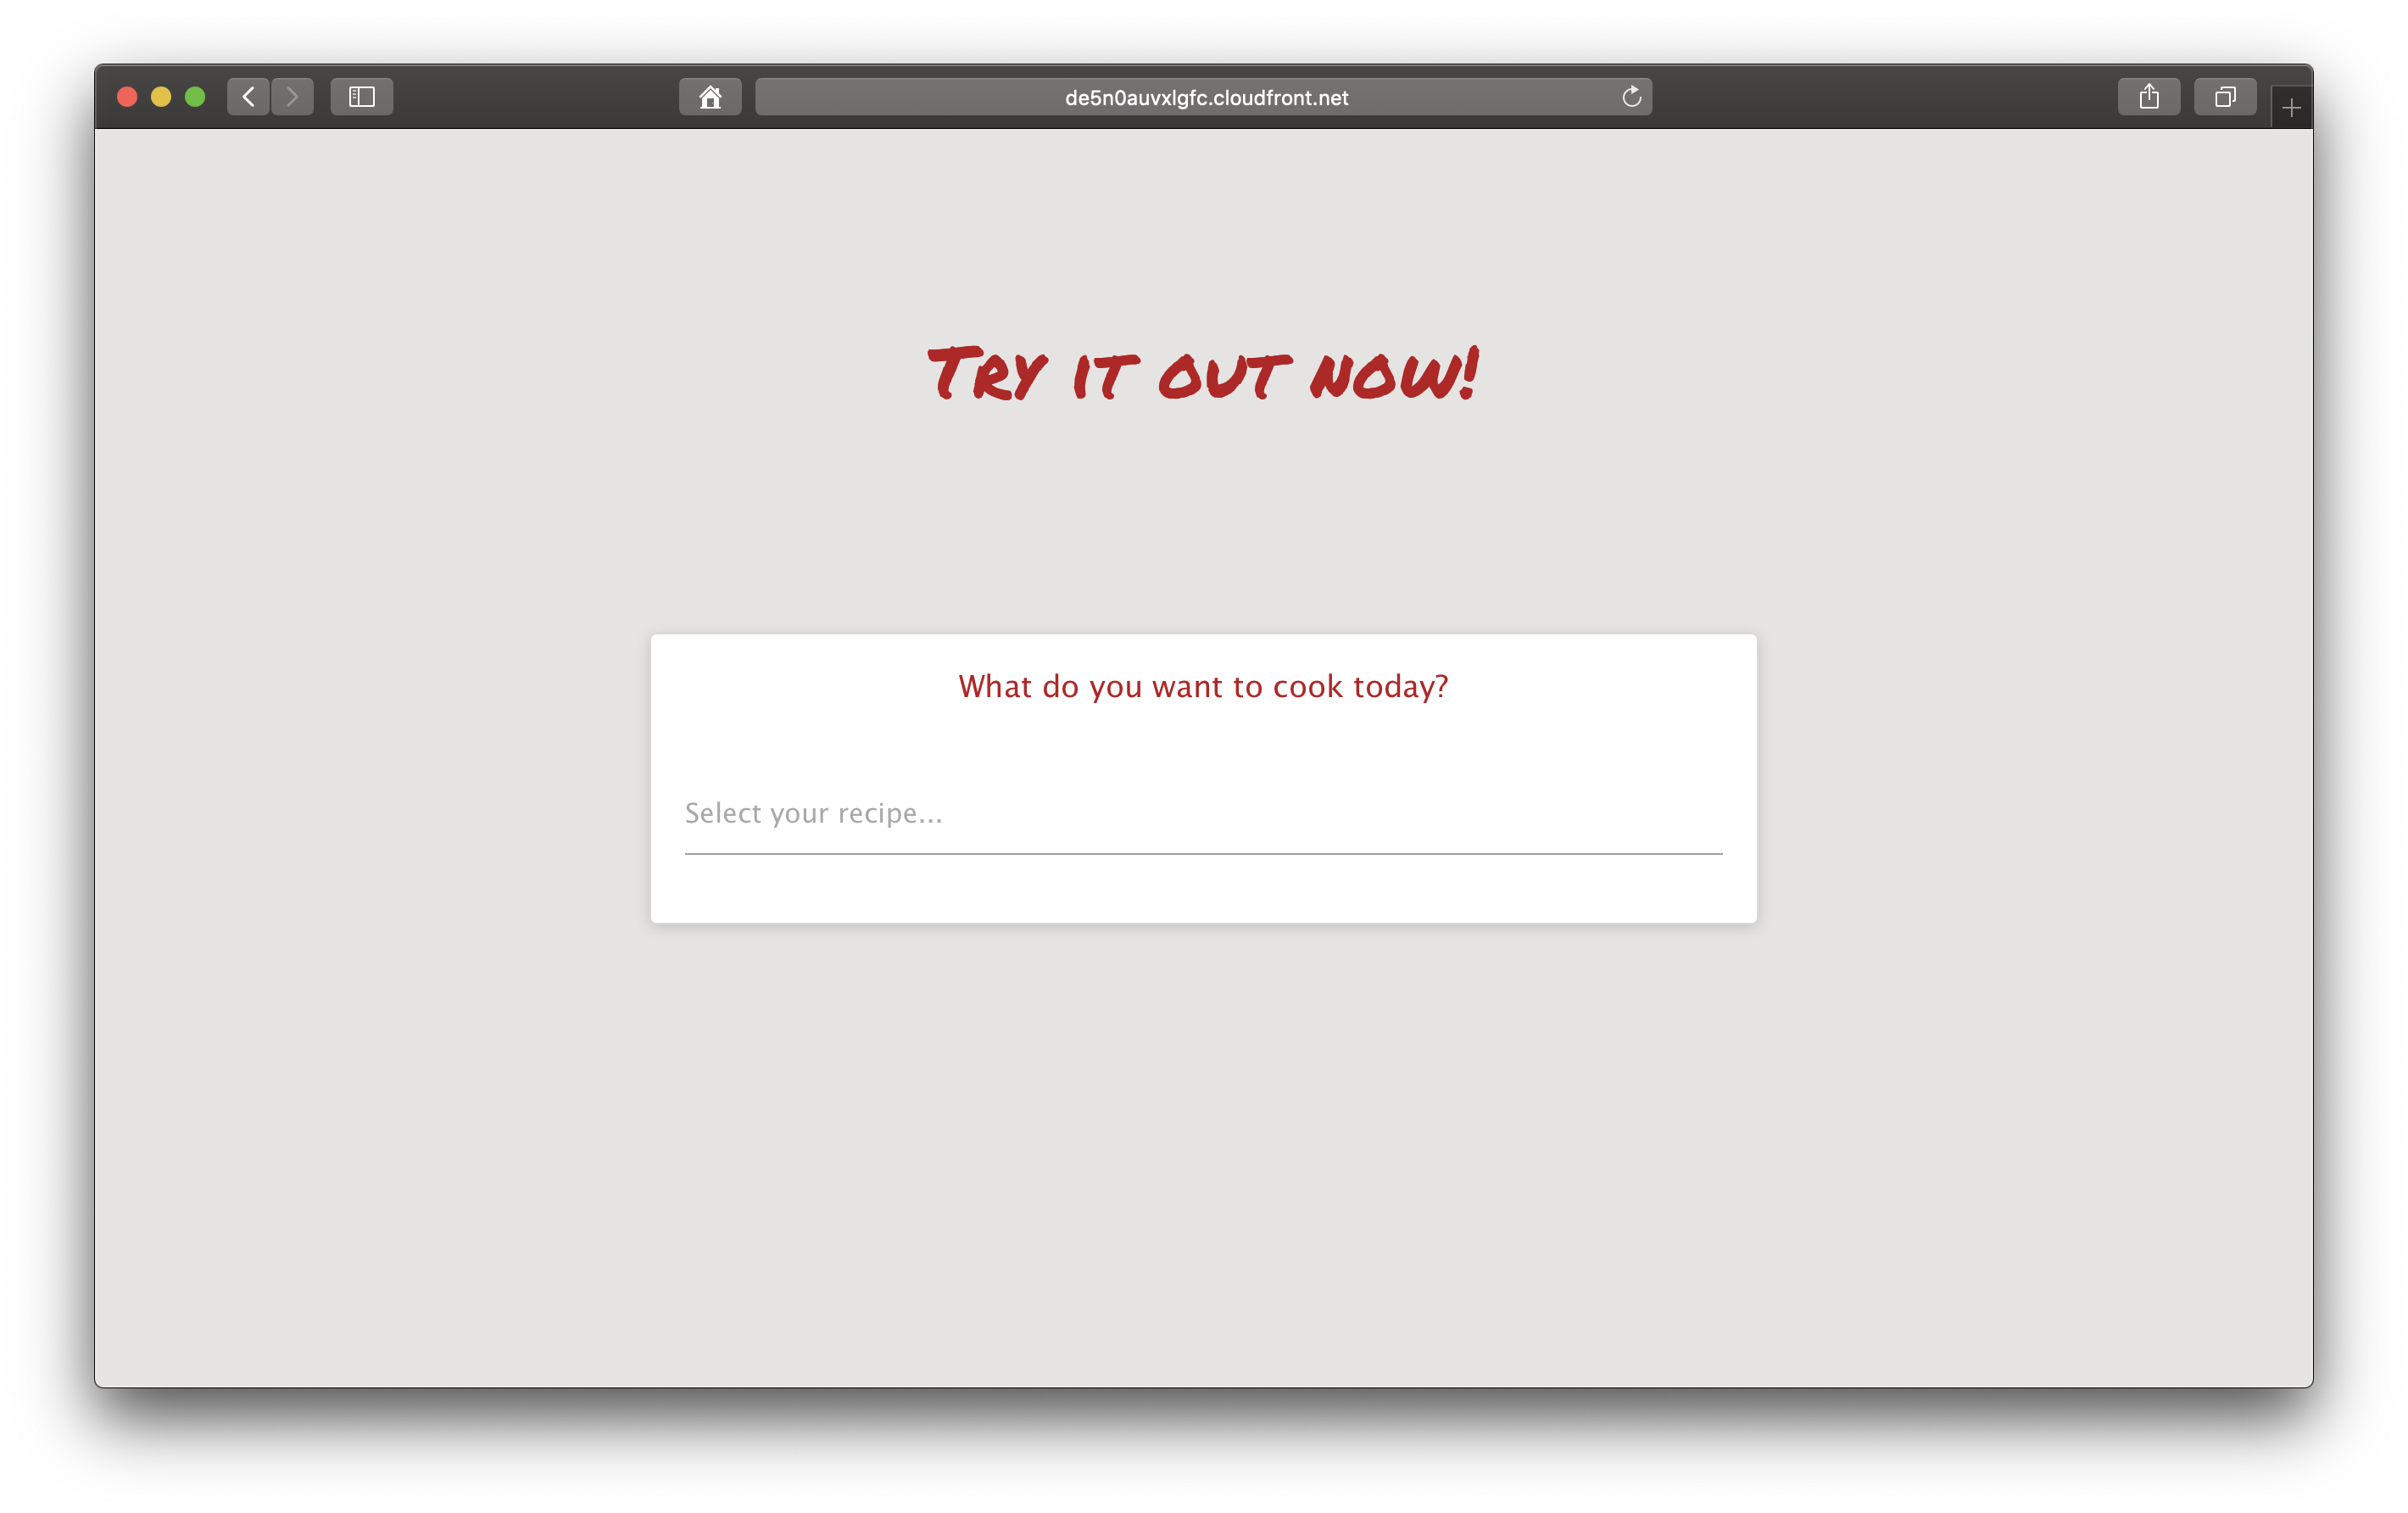
\includegraphics[scale=0.30]{Ressourcen/img/screenshots/screenshotC.png}
		\vspace{-3em}
		\caption{About-Us Subpage 4}
		\label{fig:subpage4}
	\end{center}
\end{figure}
\vspace{-3em}
Initially, a page visitor starts on our \texttt{About-Us} page, which is also accessible by clicking on the \texttt{About-Us} index tab in the navigation menu. This page is separated into four subpages and mainly serves the purpose of informing the user about Foodo's services. If a user decides to give Foodo a try by either clicking on the \texttt{Get Started} button on the first subpage (see figure \ref{fig:subpage}) or by selecting a recipe he wants to cook on the last subpage (see figure \ref{fig:subpage4}), he will be forwarded to our \texttt{Login/Registration-Page} (see next section).
\section*{Login/Registration}
\vspace{-2em}
\begin{figure}[H]
	\captionsetup{justification=centering}
	\begin{center}
		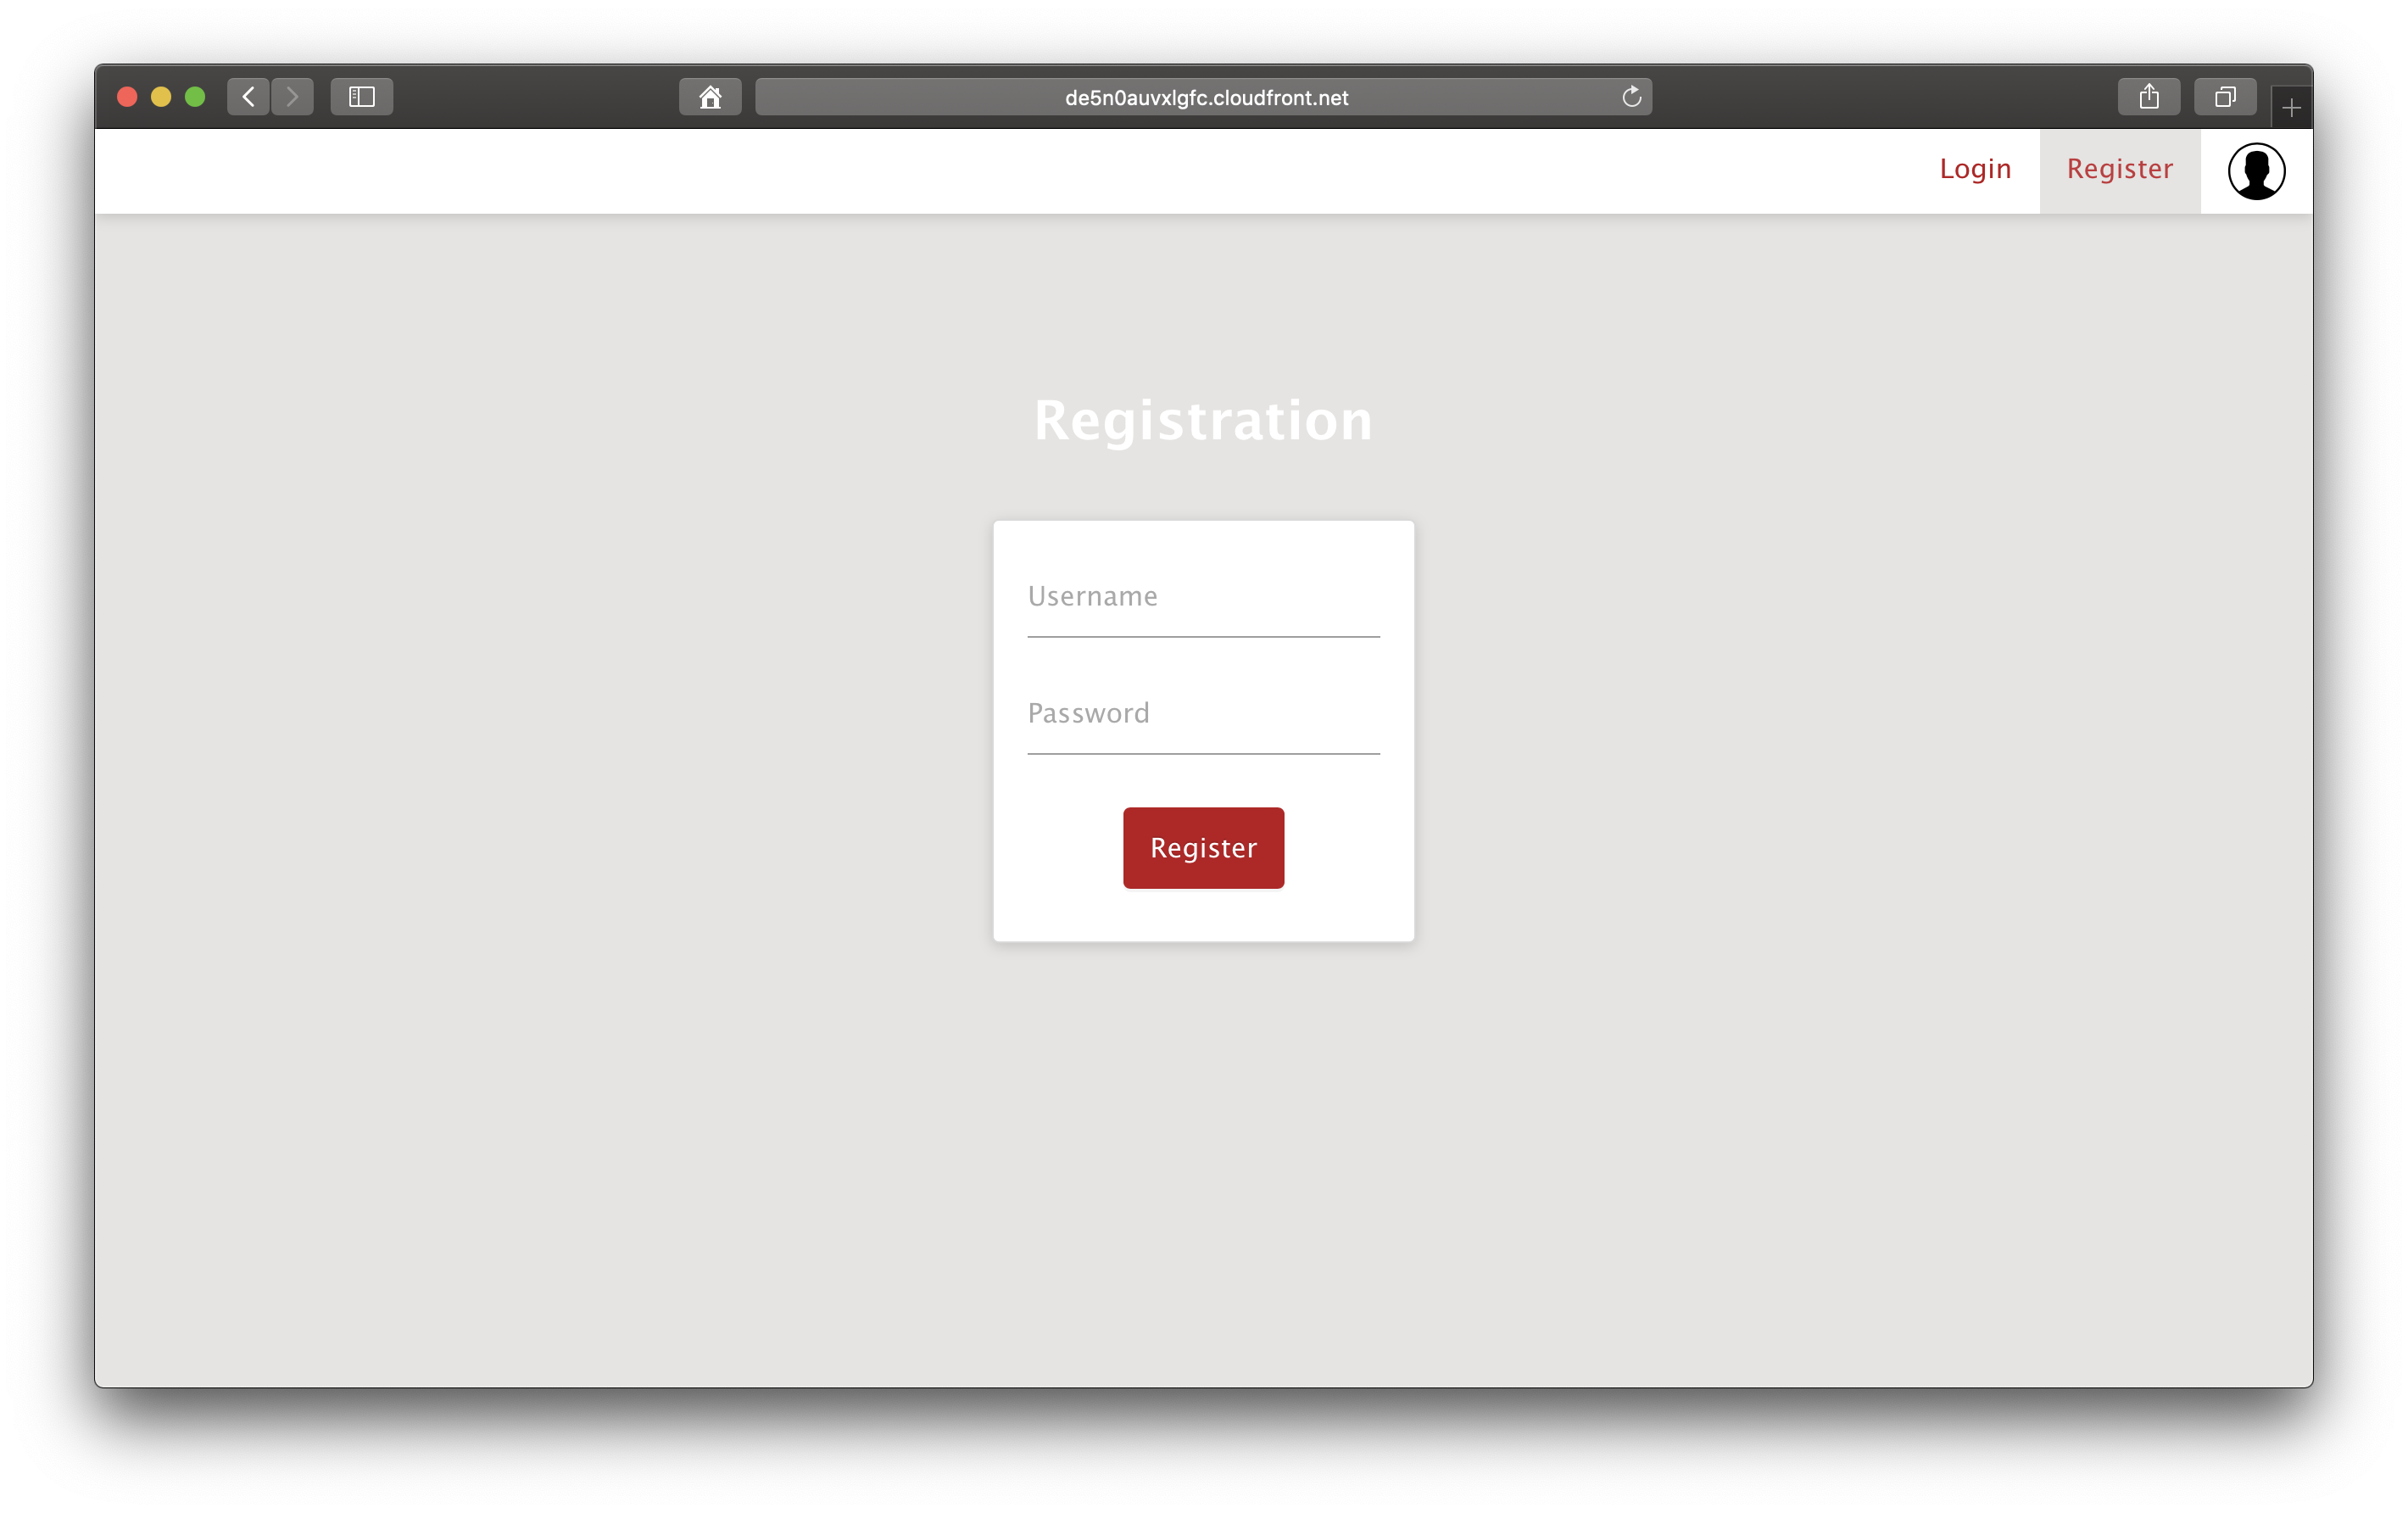
\includegraphics[scale=0.28]{Ressourcen/img/screenshots/screenshotD.png}
		\vspace{-3em}
		\caption{Registration}
		\label{fig:registration}
	\end{center}
\end{figure}
Before a user can use Foodo’s services, he first needs to create an account. Therefore, he will always be redirected to the \texttt{Login/Registration-Page} (see figure \ref{fig:registration}), when he tries to call a service URL or clicks the mentioned button or recipe selector in the previous section (\texttt{About-Us page}). By inserting an individual username, which has not been taken already, and a hopefully secure password, the user can create a new account for himself. He also has the option to login with an already registered account by clicking on \texttt{Login} in the right upper corner and inserting his previously created credentials in the following form.
\section*{Navigation bar}
\vspace{-2em}
\begin{figure}[H]
	\captionsetup{justification=centering}
	\begin{center}
		\includegraphics[scale=0.4]{Ressourcen/img/screenshots/screenshotE.png}
		\vspace{-3em}
		\caption{Navbar}
		\label{fig:navbar}
	\end{center}
\end{figure}
\vspace{-3em}
In the previous sections, there was no navigation bar at the top of the screen, as one could see in the figures. This was due to the limited options a user has without registered account. Now, after a user has logged into his account, he can find a navigation bar, shown in figure \ref{fig:navbar}. By clicking on the profile icon in the upper right corner, a menu panel will be shown with additional navigation options for the user. Overall, he has the following navigation options:
\begin{itemize}
\item \textbf{Home}: The main page of Foodo, described in the next section
\item \textbf{My Profile}: The user's settings and preferences regarding food items and nutrition; described in section Profile Page.
\item \textbf{Statistics}: The user's improvements depicted with graphics and values; described in section \texttt{Statistics}.
\item \textbf{Preferences}: This will open another small menu panel with two submenus. Clicking on \texttt{Languages} will again open another small menu panel, where the user can choose between the offered languages (currently only English and German). Clicking on \texttt{Password} will direct the user to a form, where he can insert his new password.
\item \textbf{About}: This will direct the user to the \texttt{About-Page} again.
\item \textbf{Logout}: This is quite self explanatory and will logout the user from his current account.
\end{itemize}
\section*{Home Page}
\vspace{-2em}
\begin{figure}[H]
	\captionsetup{justification=centering}
	\begin{center}
		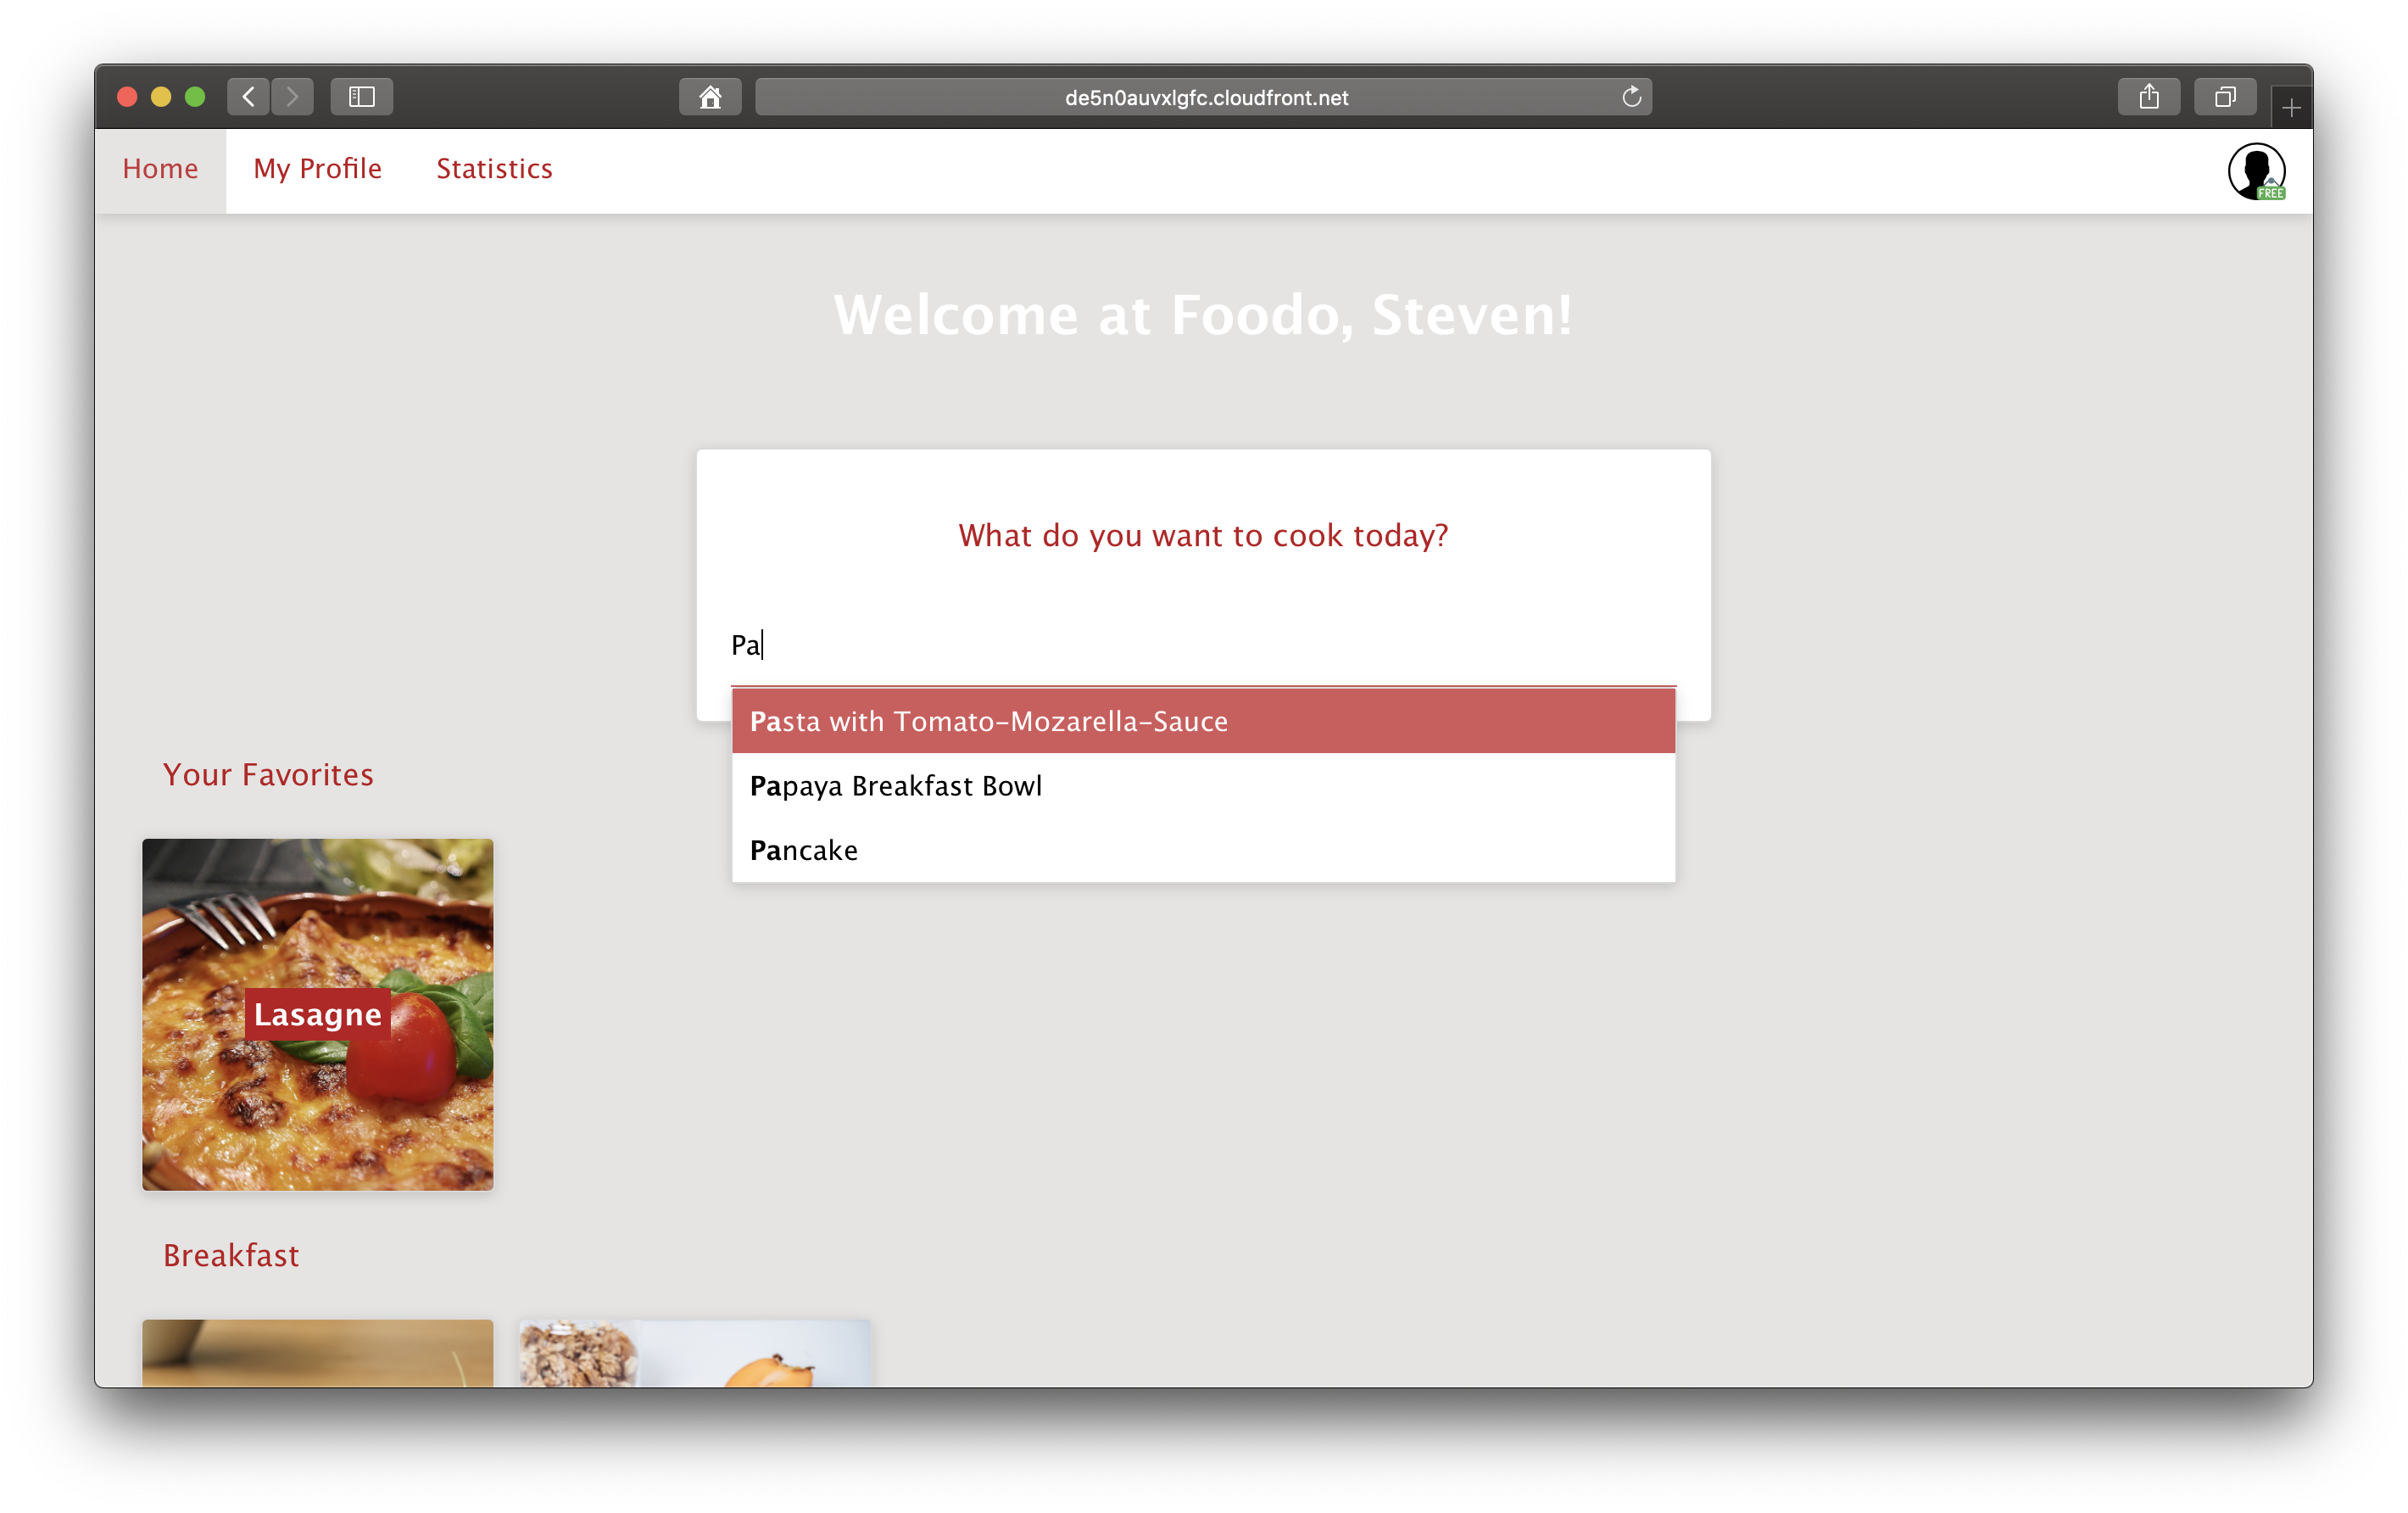
\includegraphics[scale=0.30]{Ressourcen/img/screenshots/screenshotF.png}
		\vspace{-3em}
		\caption{Home page recipe selector }
		\label{fig:recipeSelector}
	\end{center}
\end{figure}
\vspace{-2em}
\begin{figure}[H]
	\captionsetup{justification=centering}
	\begin{center}
		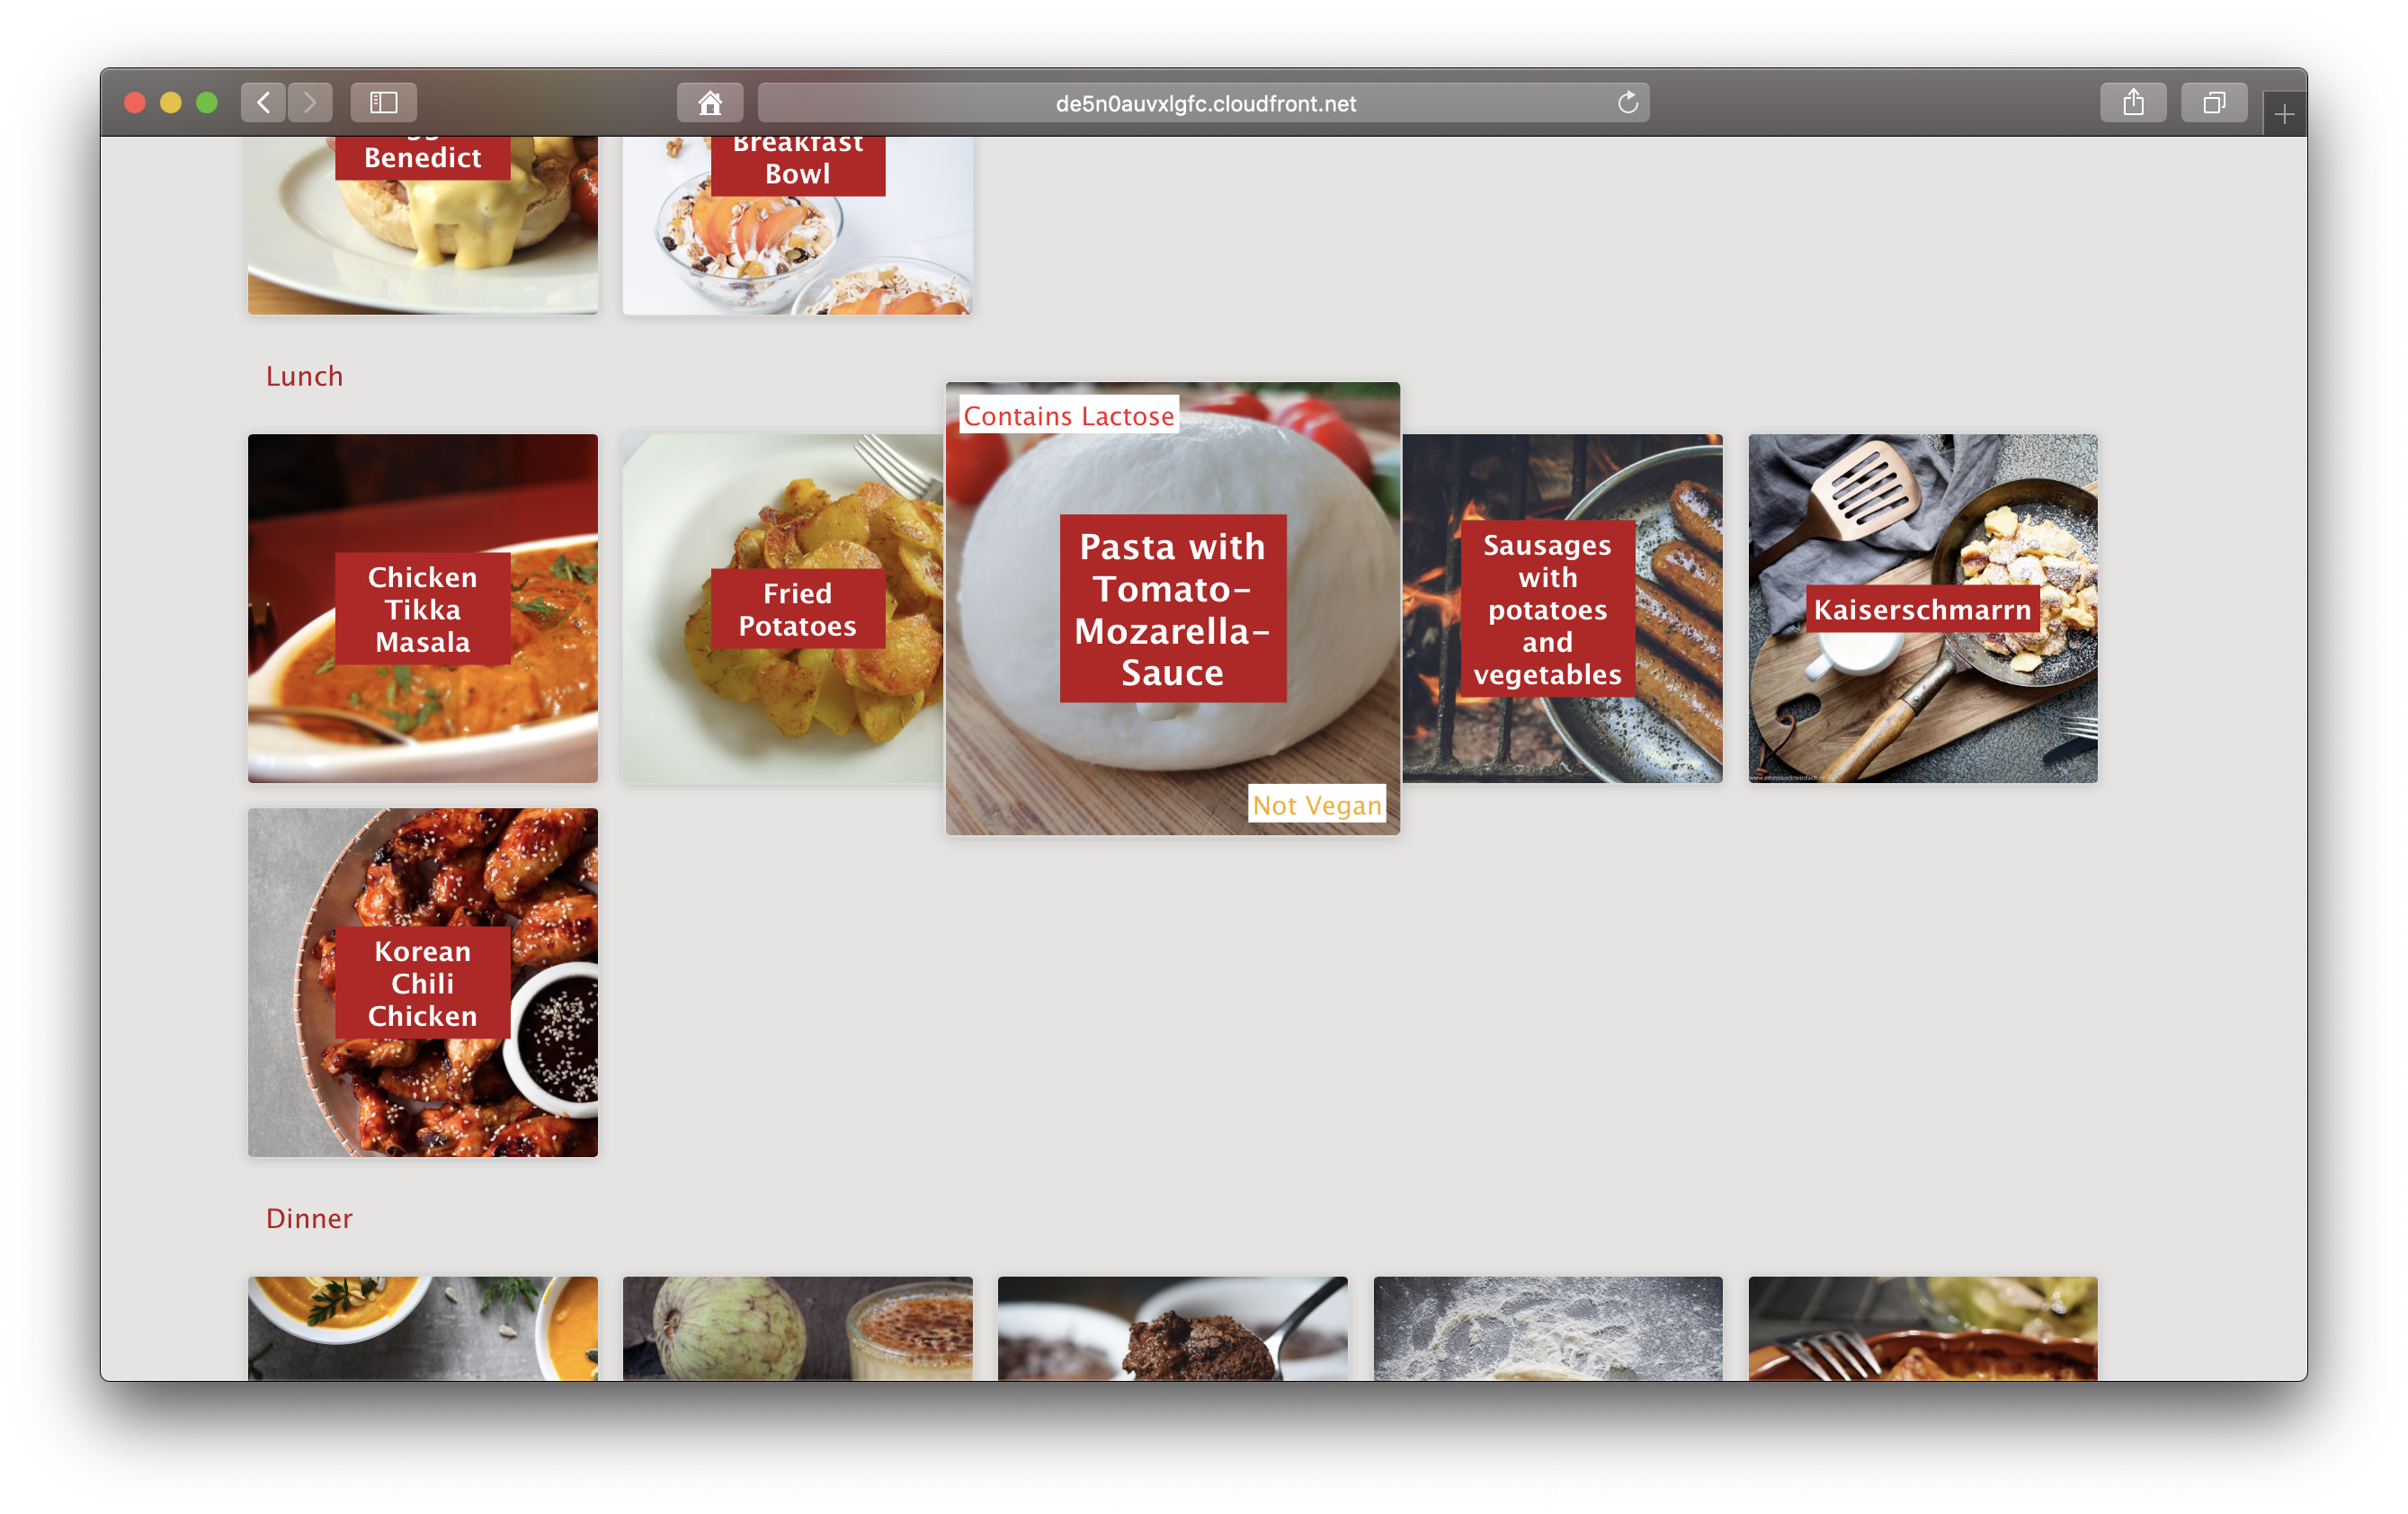
\includegraphics[scale=0.30]{Ressourcen/img/screenshots/screenshotG.png}
		\vspace{-3em}
		\caption{Home page recipe tiles}
		\label{fig:recipeTiles}
	\end{center}
\end{figure}
This is the main page of our application, where the user can browse through a variety of recipes. To find a recipe he likes, he can either click on the \texttt{'Select your recipe…'} input field and select a recipe out of the appearing list (see figure \ref{fig:recipeSelector}) or browse through our displayed recipes below (see figure \ref{fig:recipeTiles}). These are categorized into four standard groups and two categories that match your lifestyle and allergies:
\clearpage
\begin{itemize}
\item Your Favorites
\item Breakfast
\item Lunch
\item Dinner
\item Tolerated recipes (allergy-based)
\item Lifestyle (e.g. Vegan, Vegetarian)
\end{itemize}	
However, before the user can start the substitution process, he is advised to go to his personal preferences and select at least a personal nutrition goal. This instruction is also shown in a yellow box, as shown in figure \ref{fig:profilesetting}.

\vspace{-1em}
\begin{figure}[H]
	\captionsetup{justification=centering}
	\centering
	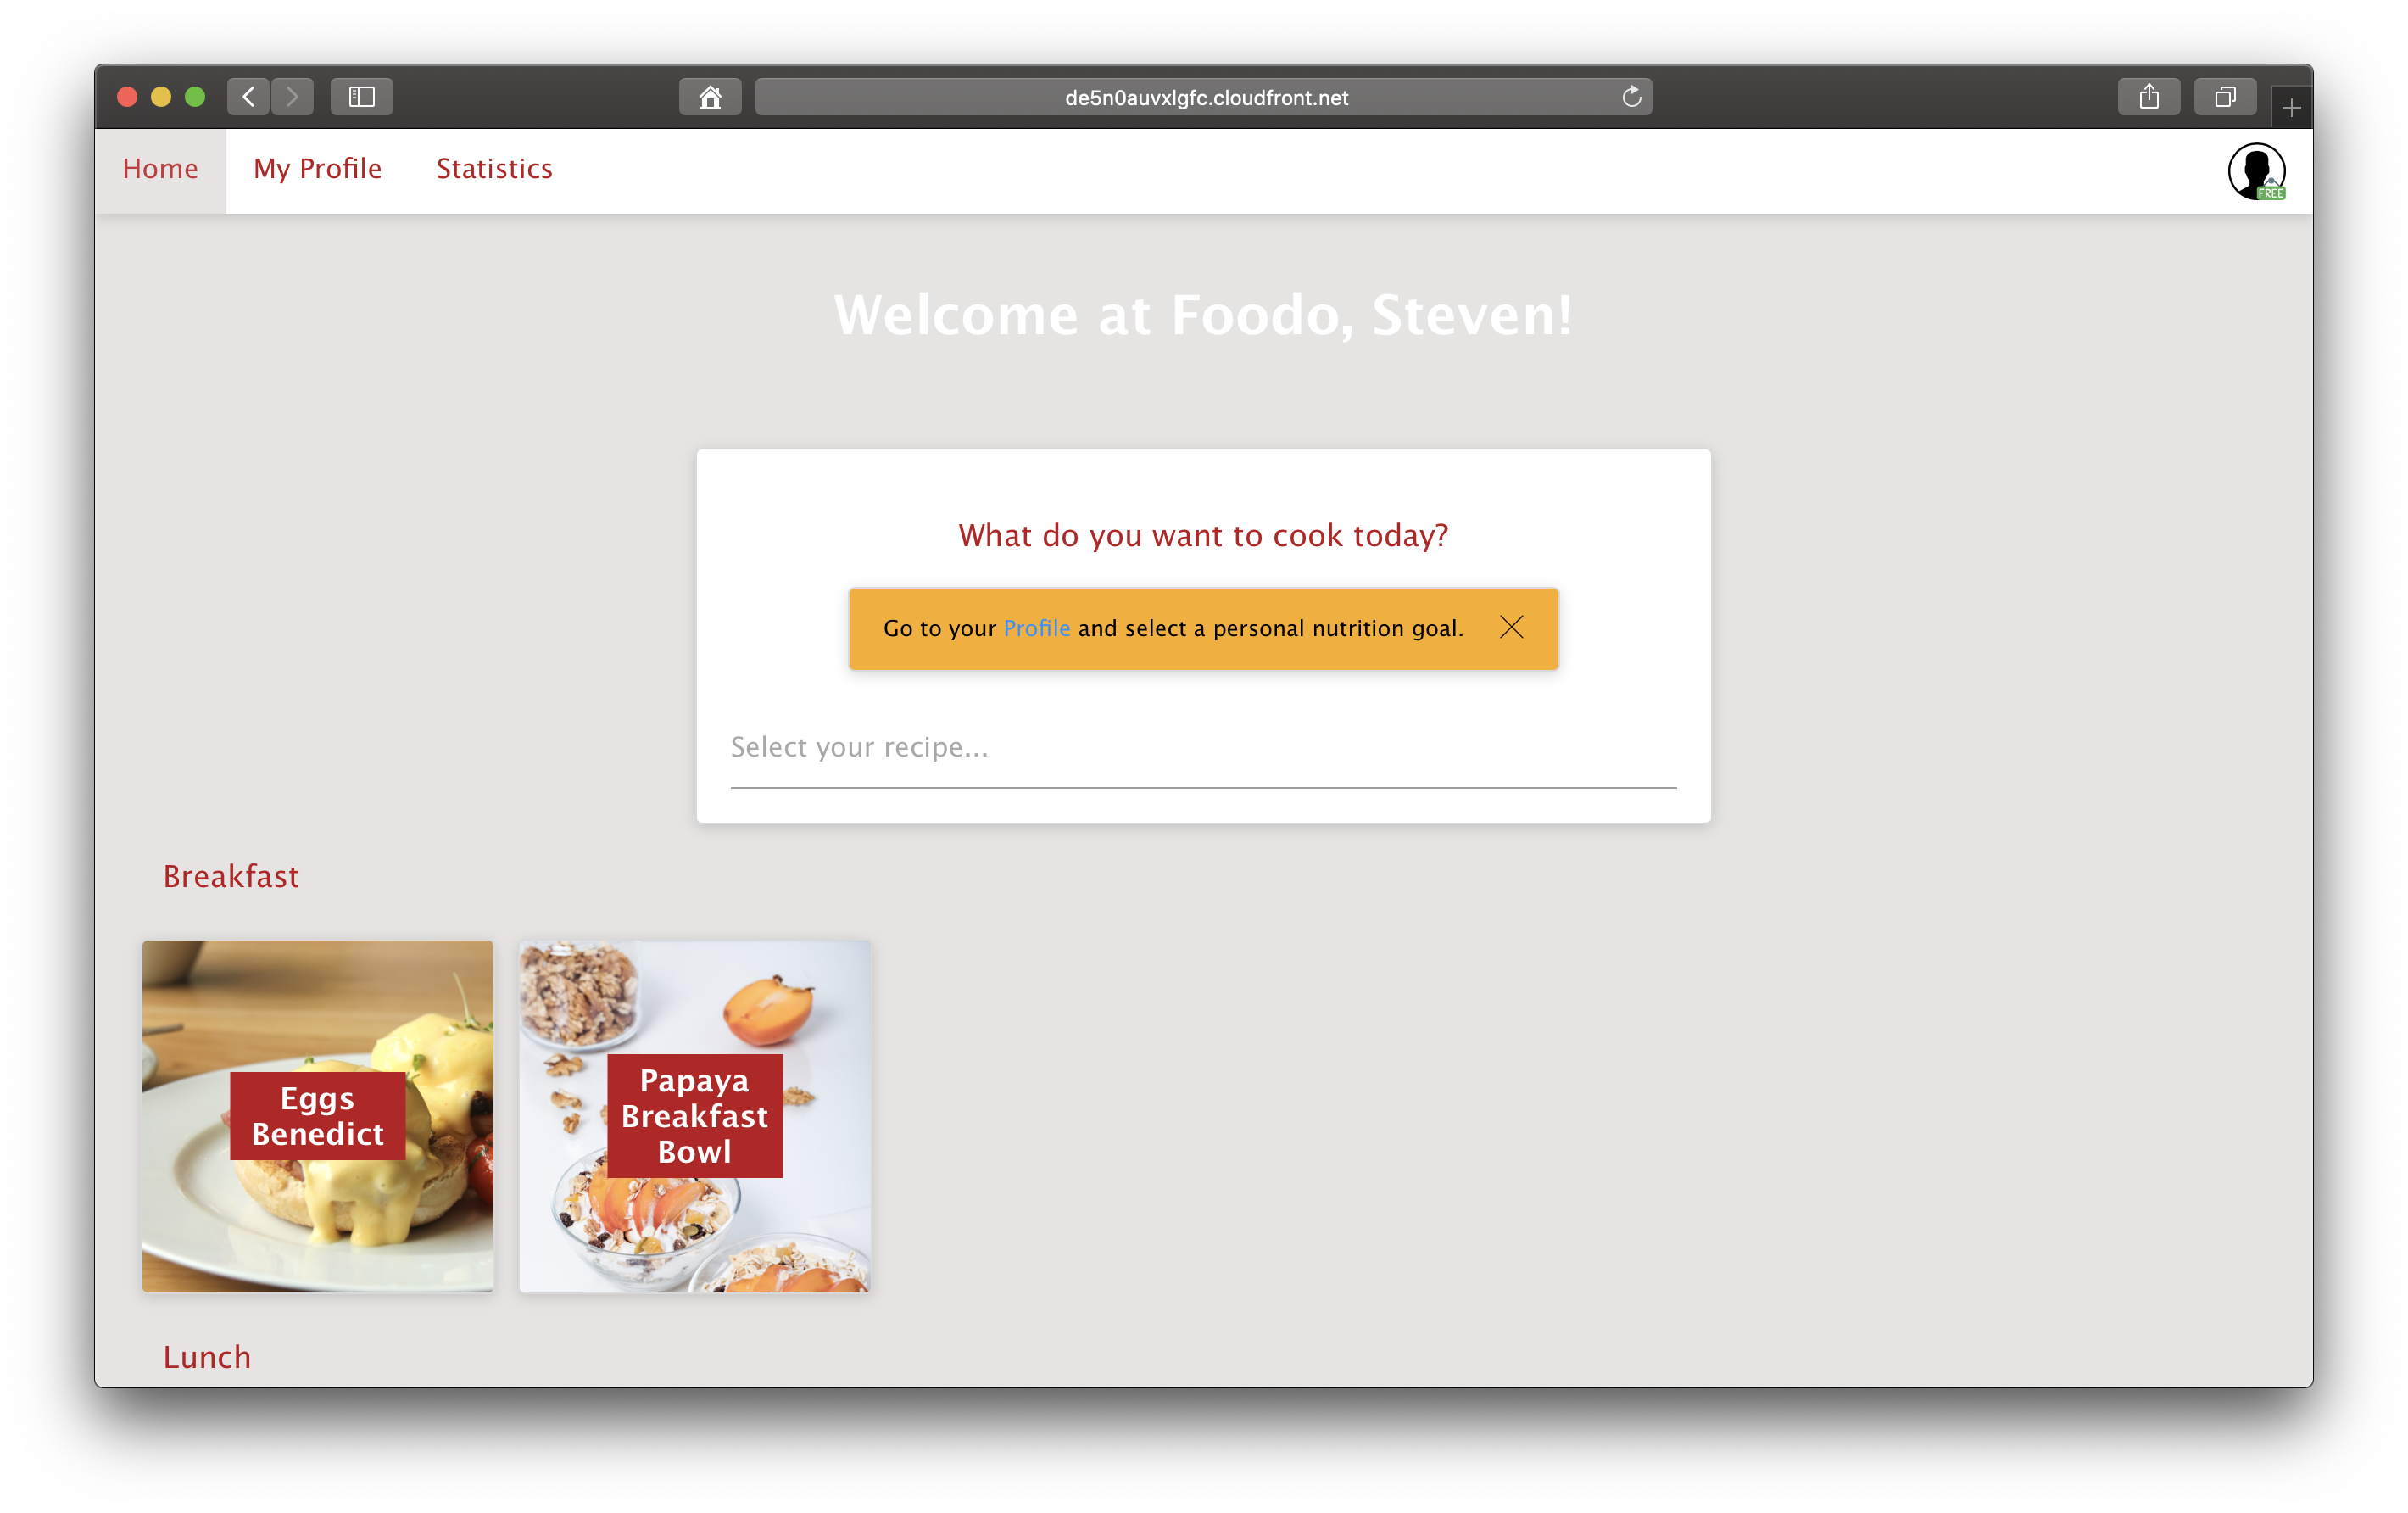
\includegraphics[scale=0.30]{Ressourcen/img/screenshots/screenshot41.png}
	\vspace{-3em}
	\caption{Profile settings for user}
	\label{fig:profilesetting}
\end{figure}

\section*{Recipe detail view}
\vspace{-1em}
\begin{figure}[H]
	\captionsetup{justification=centering}
	\centering
		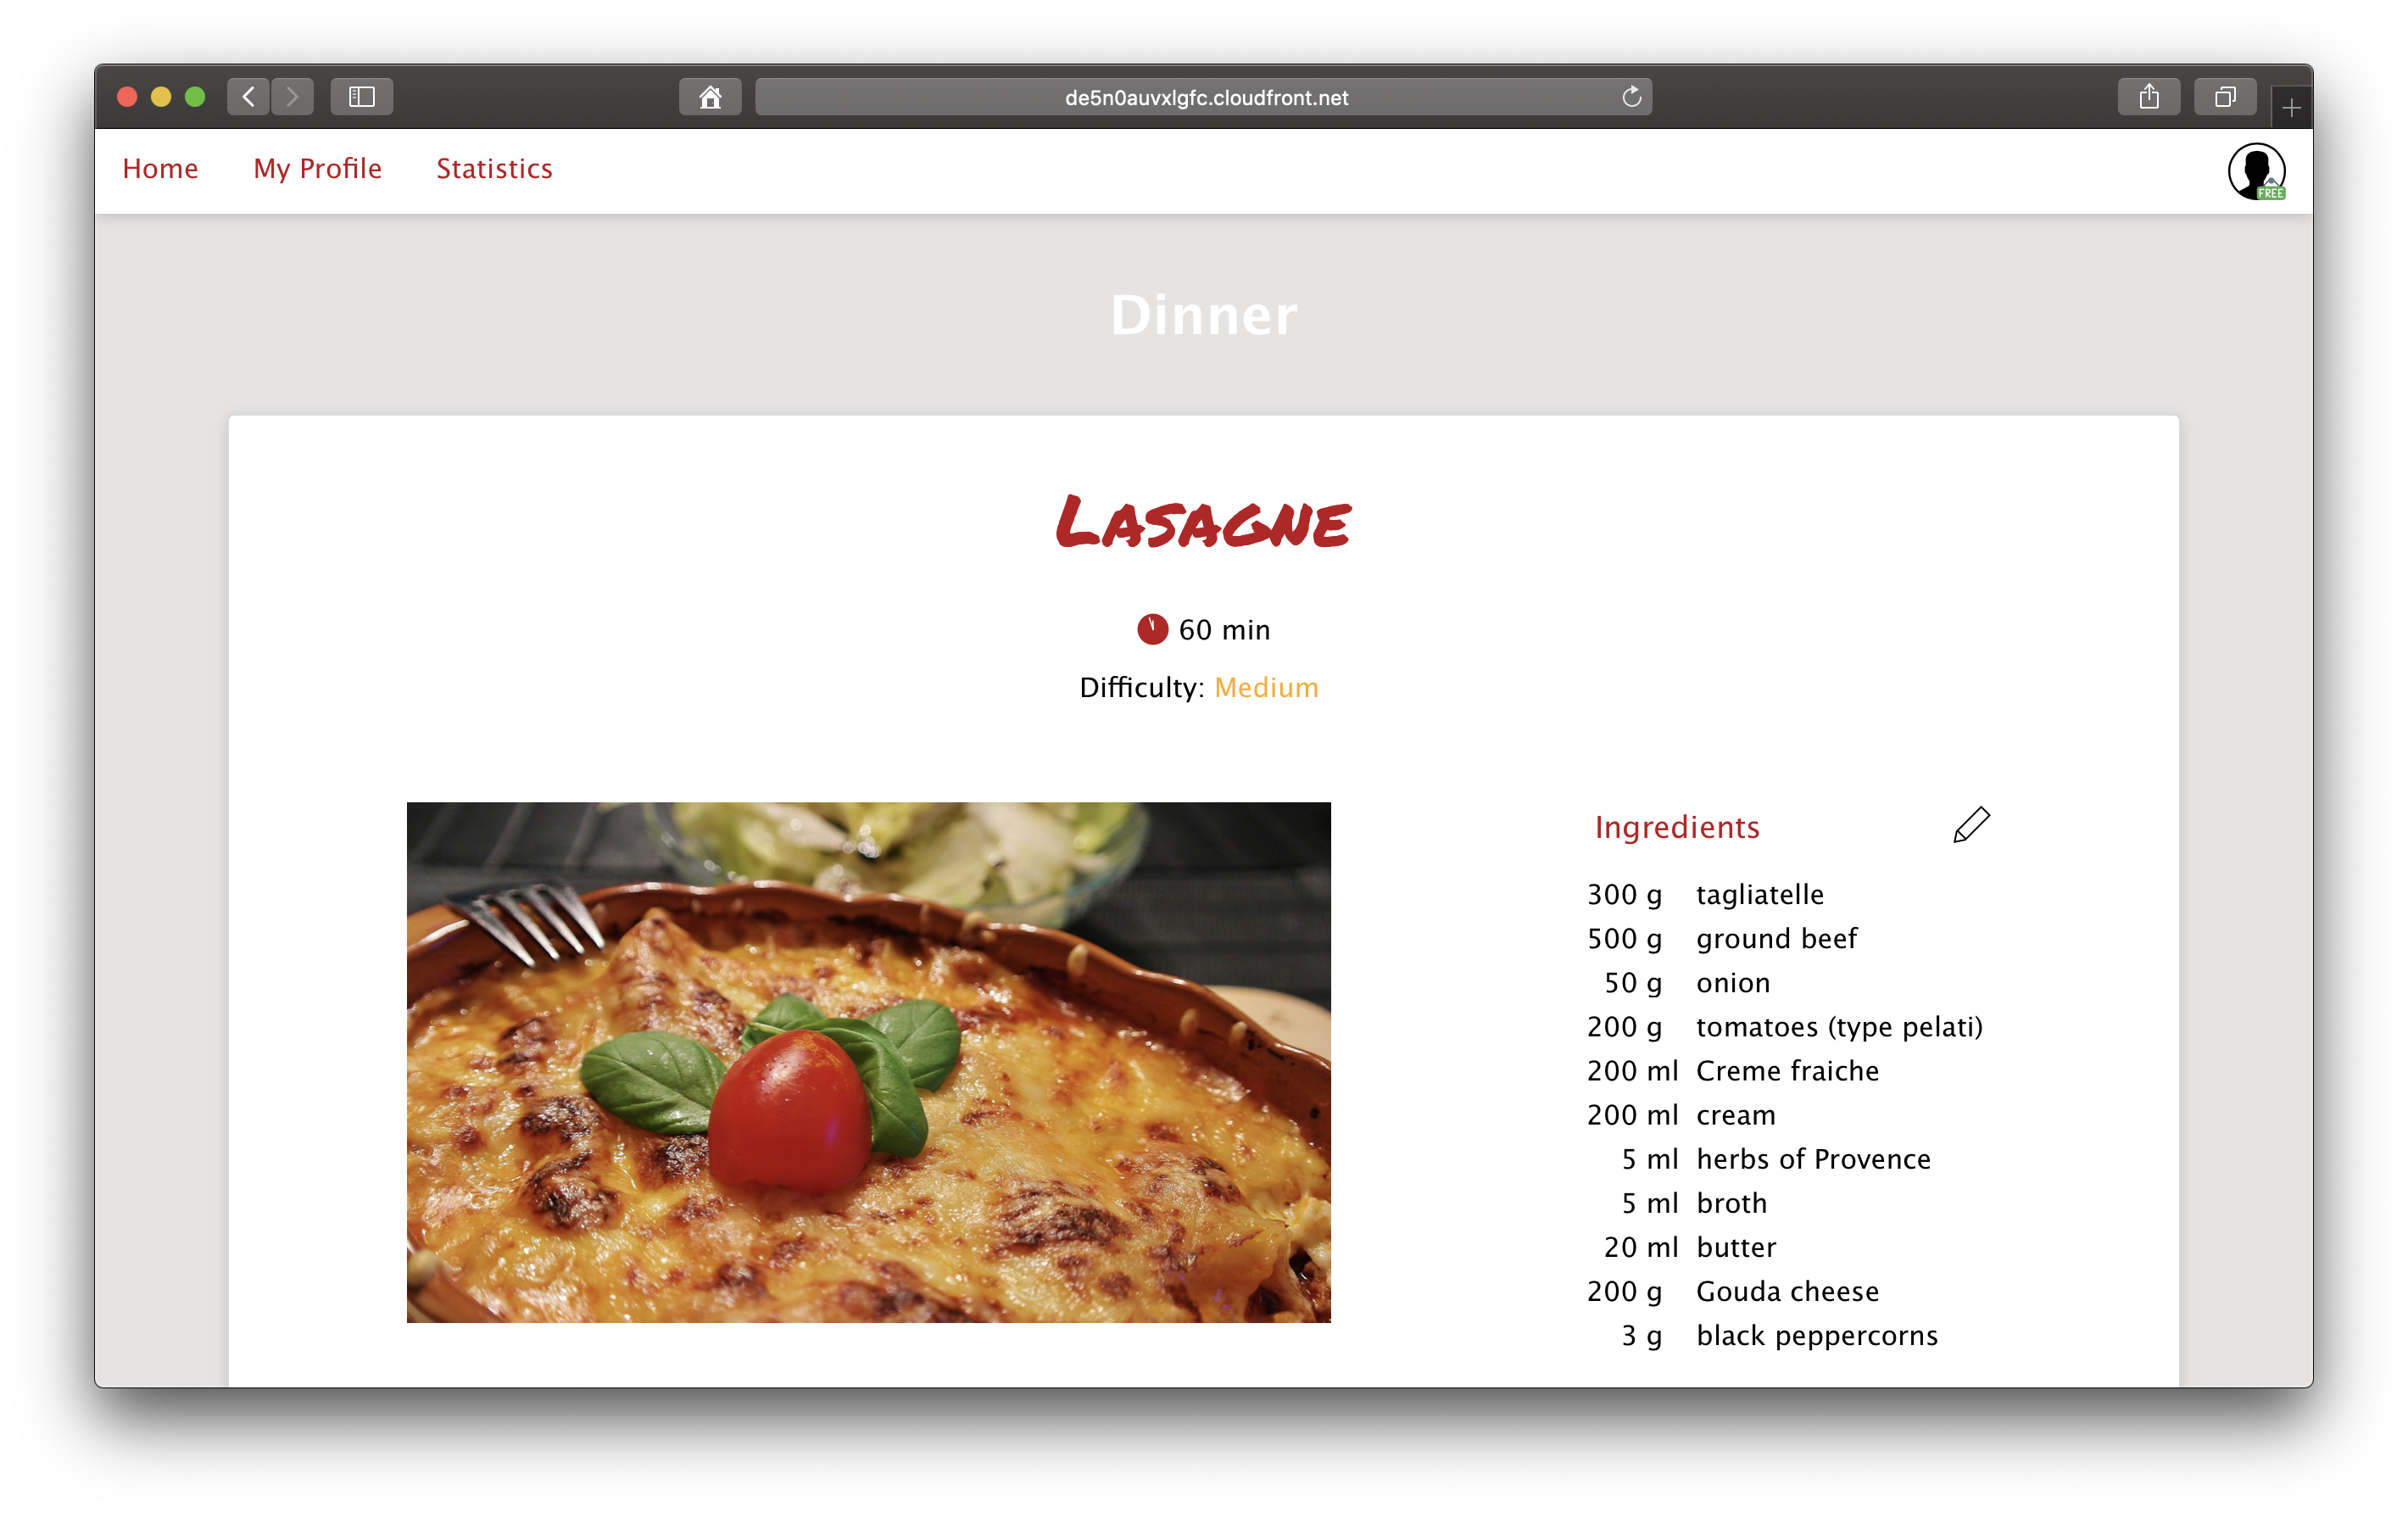
\includegraphics[scale=0.25]{Ressourcen/img/screenshots/screenshotH.png}
		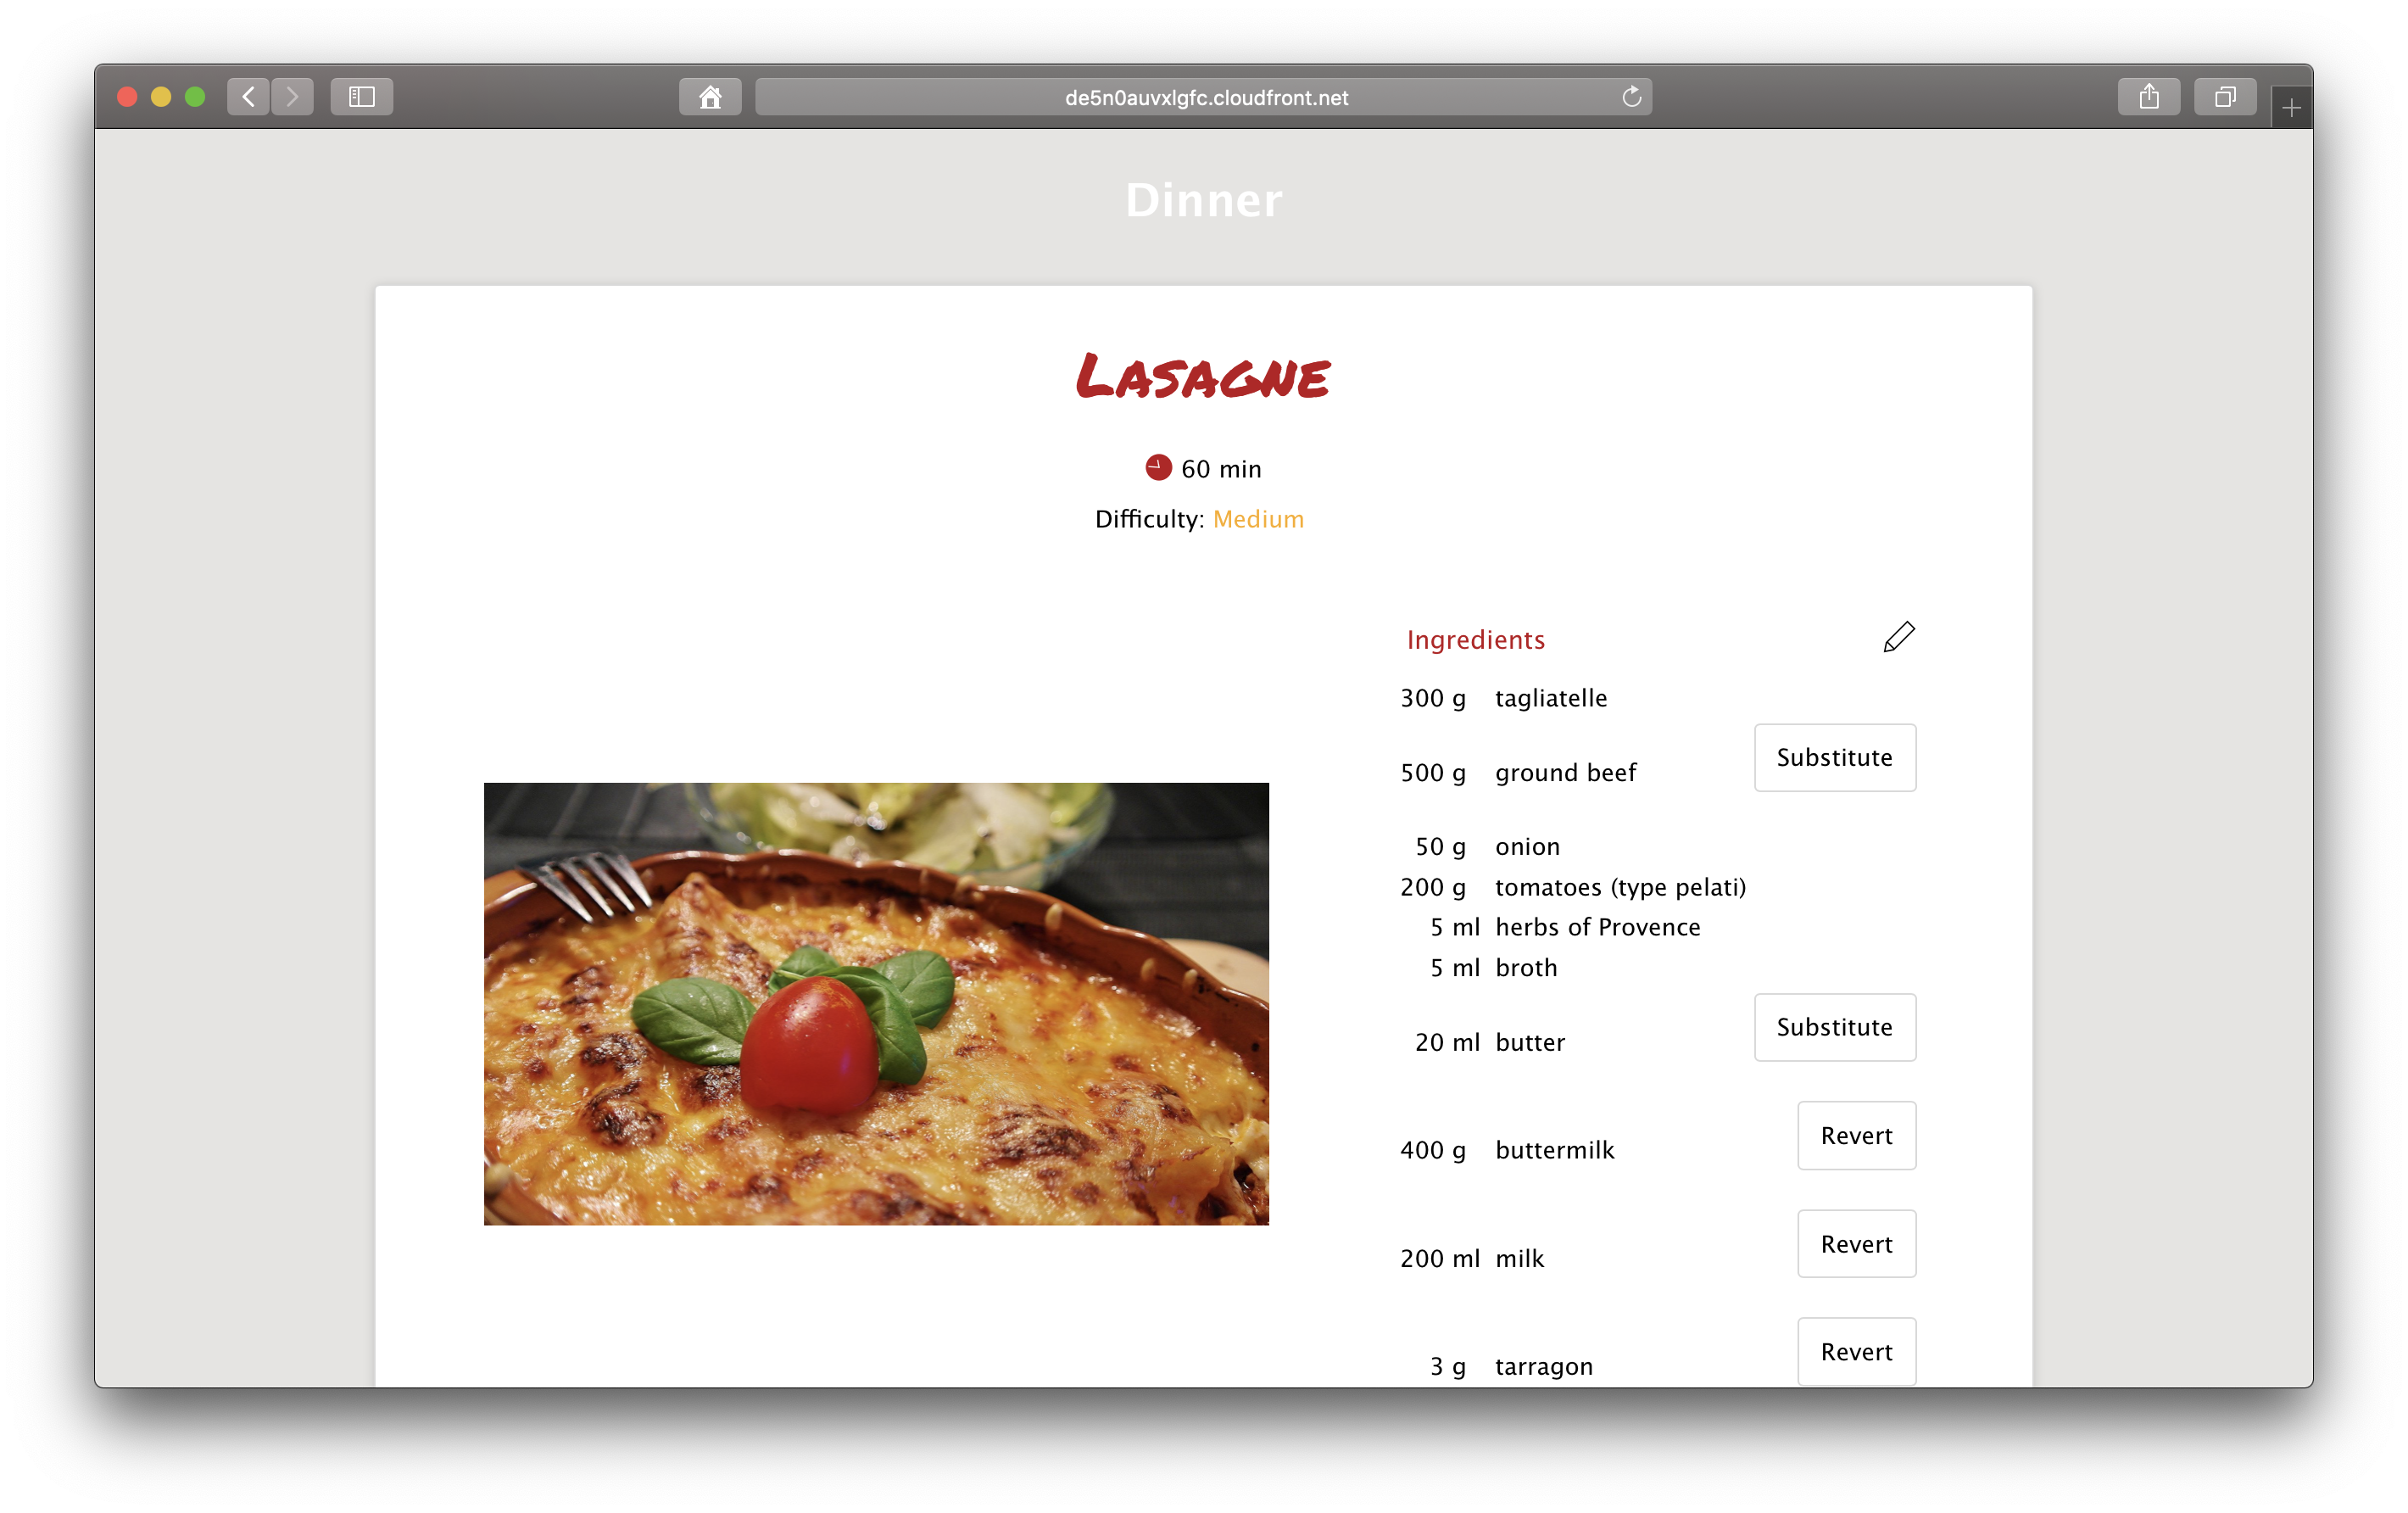
\includegraphics[scale=0.25]{Ressourcen/img/screenshots/screenshotI.png}
		\vspace{-1em}
		\caption{Recipe detail view without and with selected user goal}
		\label{fig:recipeDetail}
\end{figure}
\vspace{-2em}
The first part of the detailed recipe overview consists of a picture and a list of ingredients. Depending on whether the user already selected his personal goal, he either sees the first or second view depicted in figure \ref{fig:recipeDetail}. For those ingredients, where there exists a better substitute in our database based on the nutriscore, a \texttt{Substitute} button will be displayed. By clicking on it, the user can select a suitable substitute as shown in figure \ref{fig:substitute}. (You can find more information regarding the substitution algorithm in chapter \emph{\ref{algorithm}  Algorithm}). In the newly opened window he can see his current NutriScore and possible alternatives for the selected ingredients together with their individual NutriScore. If the user already substituted an ingredient with another one and wishes to revert the substitution, he can click on the meanwhile displayed \texttt{Revert} button next to the substitute he wishes to revert. 
There is also the option to personalise the recipe by clicking on the pencil icon on top of the ingredients list. This will open the window shown in figure \ref{fig:personalisation}, where the user can add or remove current ingredients.

\vspace{-1em}
\begin{figure}[H]
	\captionsetup{justification=centering}
	\begin{center}
		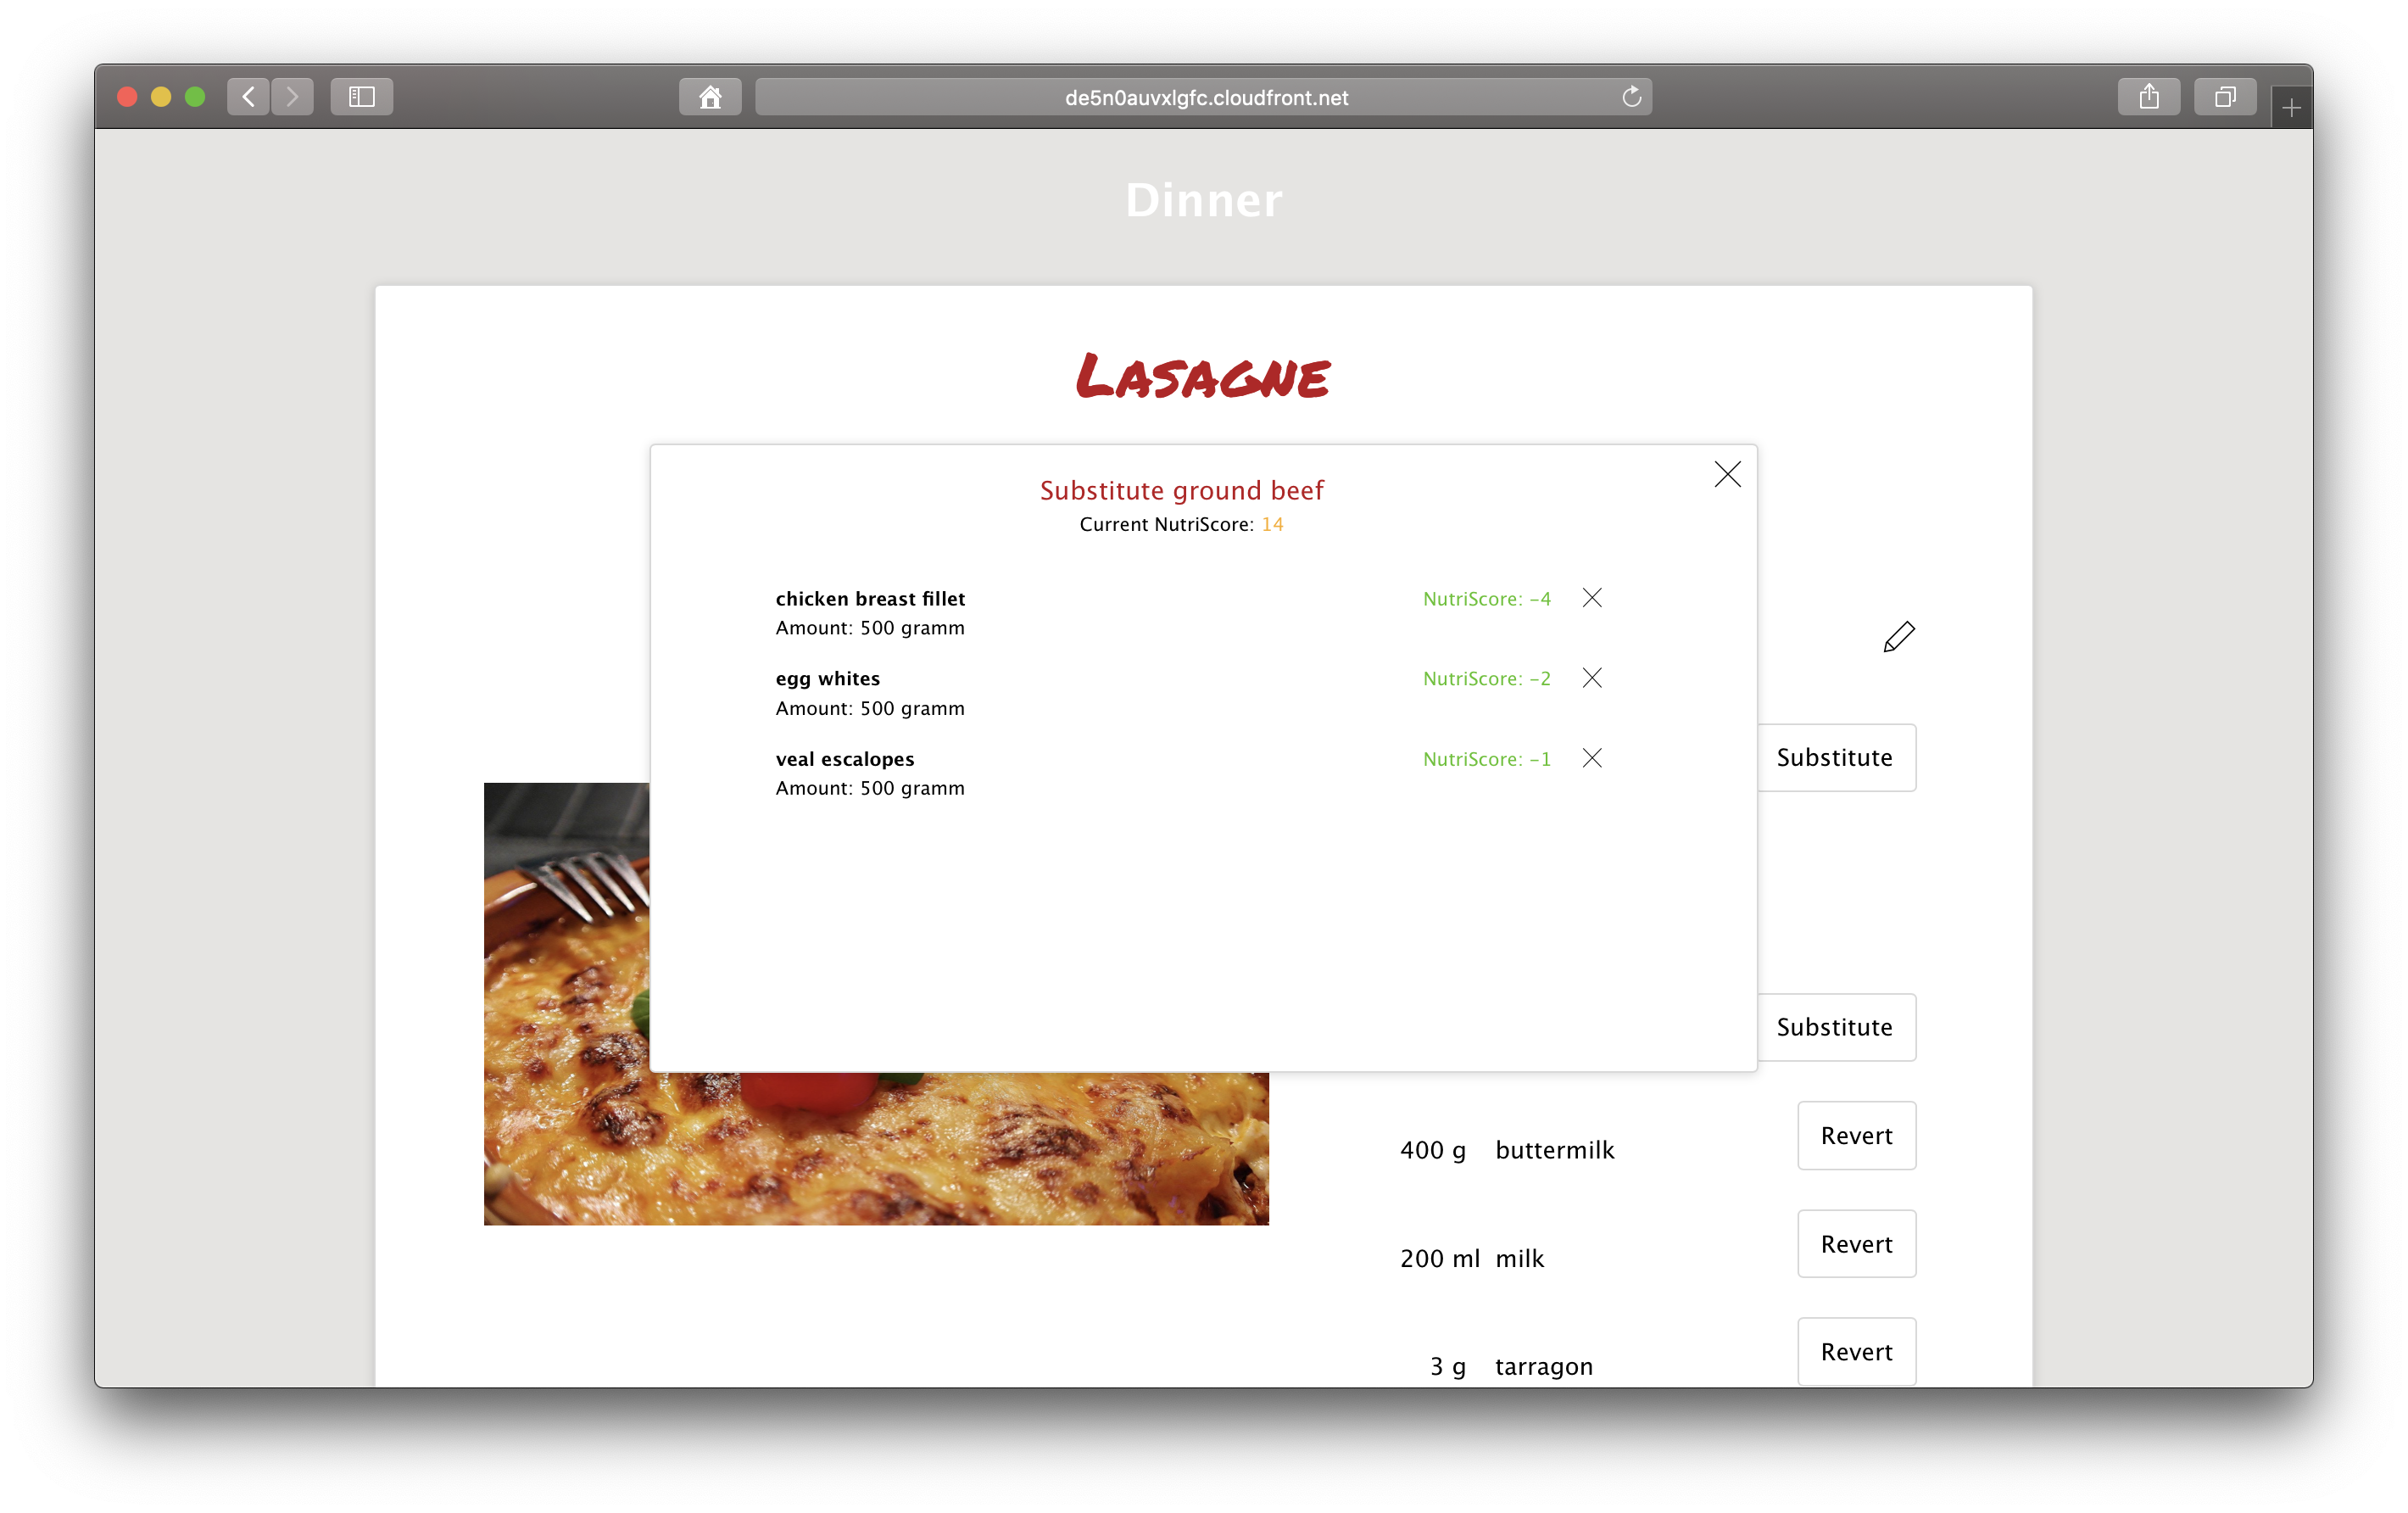
\includegraphics[scale=0.28]{Ressourcen/img/screenshots/screenshotJ.png}
		\vspace{-3em}
		\caption{Potential substitutes for beef}
		\label{fig:substitute}
	\end{center}
\end{figure}

\vspace{-2em}
\begin{figure}[H]
	\captionsetup{justification=centering}
	\begin{center}
		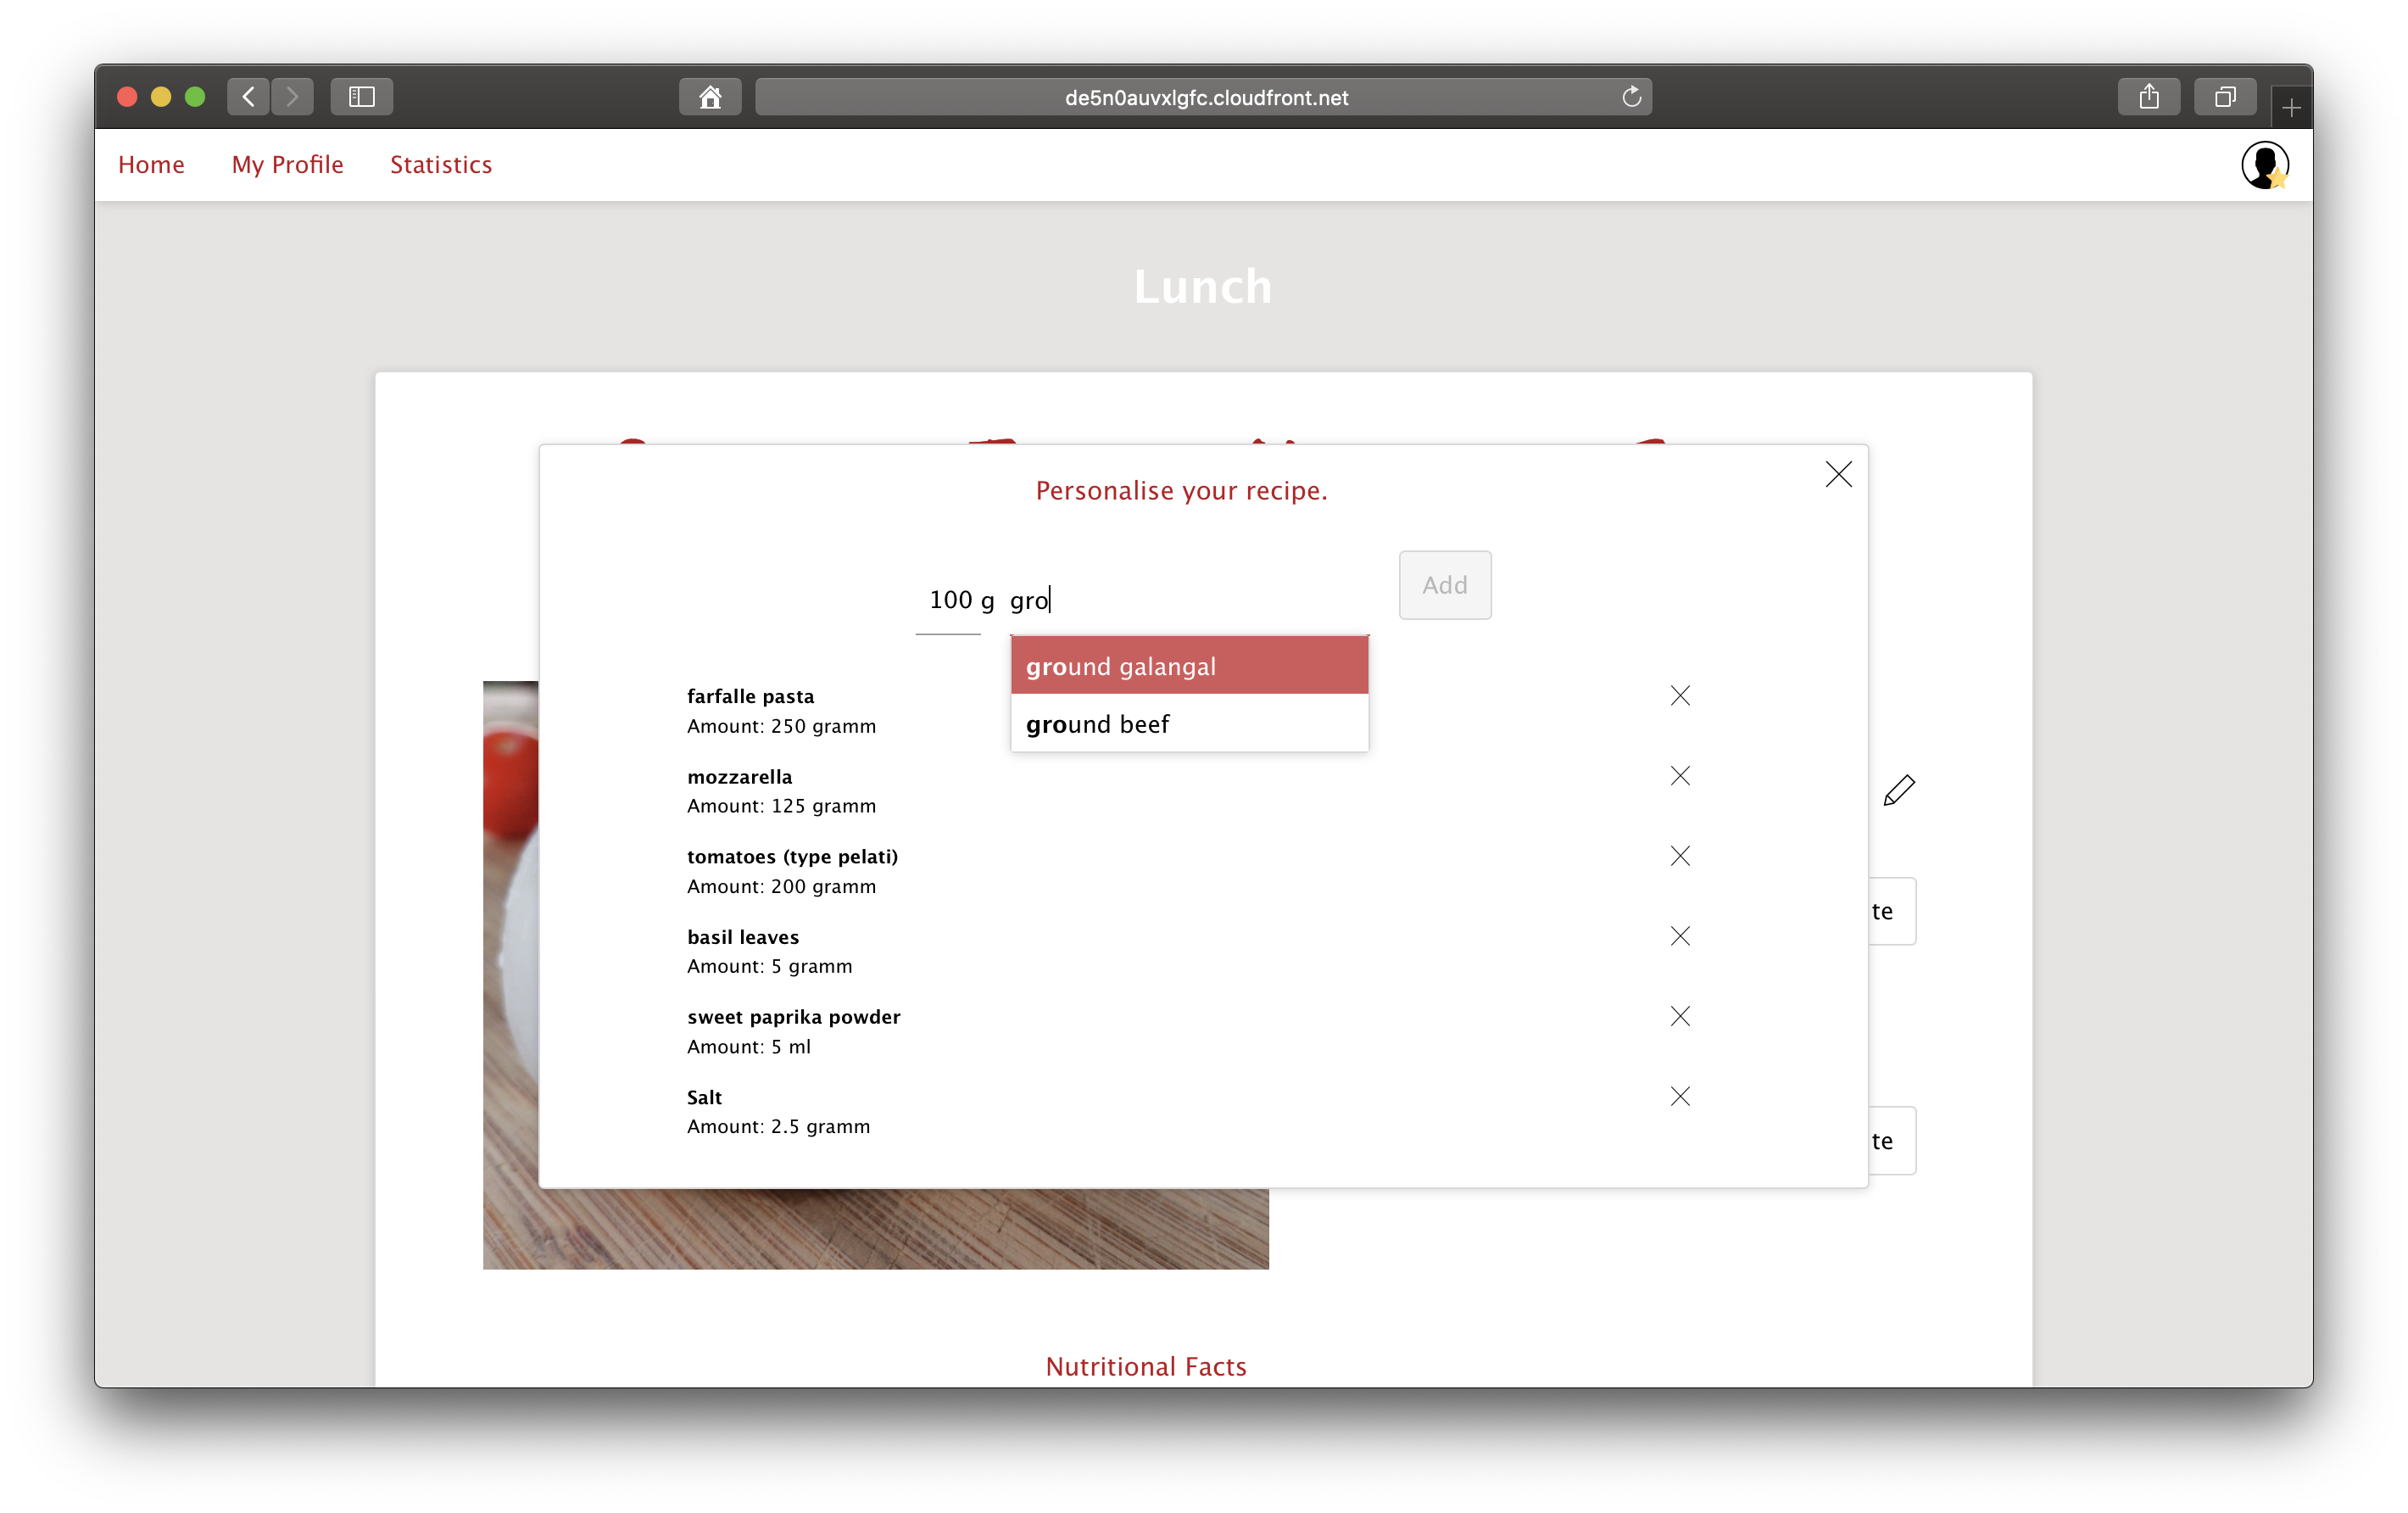
\includegraphics[scale=0.28]{Ressourcen/img/screenshots/screenshotK.png}
		\vspace{-3em}
		\caption{Recipe personalisation}
		\label{fig:personalisation}
	\end{center}
\end{figure}

Below the recipe details, the user can also find some nutritional facts consisting of graphs and statistics regarding the (modified) recipe. He can scroll through three different representations of the nutritional composition of his recipe:
\begin{itemize}
\item \textbf{Pie chart}: This is the initially shown diagram, which merely displays the ratio of carbohydrates, fats and proteins without additional numbers (see figure \ref{fig:detailedStatistics} - first screenshot).
\item \textbf{Table}: Here, the user can find the most important components of the nutrition table (see figure \ref{fig:detailedStatistics} - second screenshot).
\item \textbf{Bar graph}: This graph shows the most important nutrition components in percentage of the optimal daily intake of an adult based on the (Quelle einbinden, EU Guidelines). It also shows how much percent the user improved or deteriorated his recipe with the current substitutions (see figure \ref{fig:detailedStatistics} - third screenshot).
\end{itemize}

\begin{figure}[H]
	\captionsetup{justification=centering}
	\begin{center}
		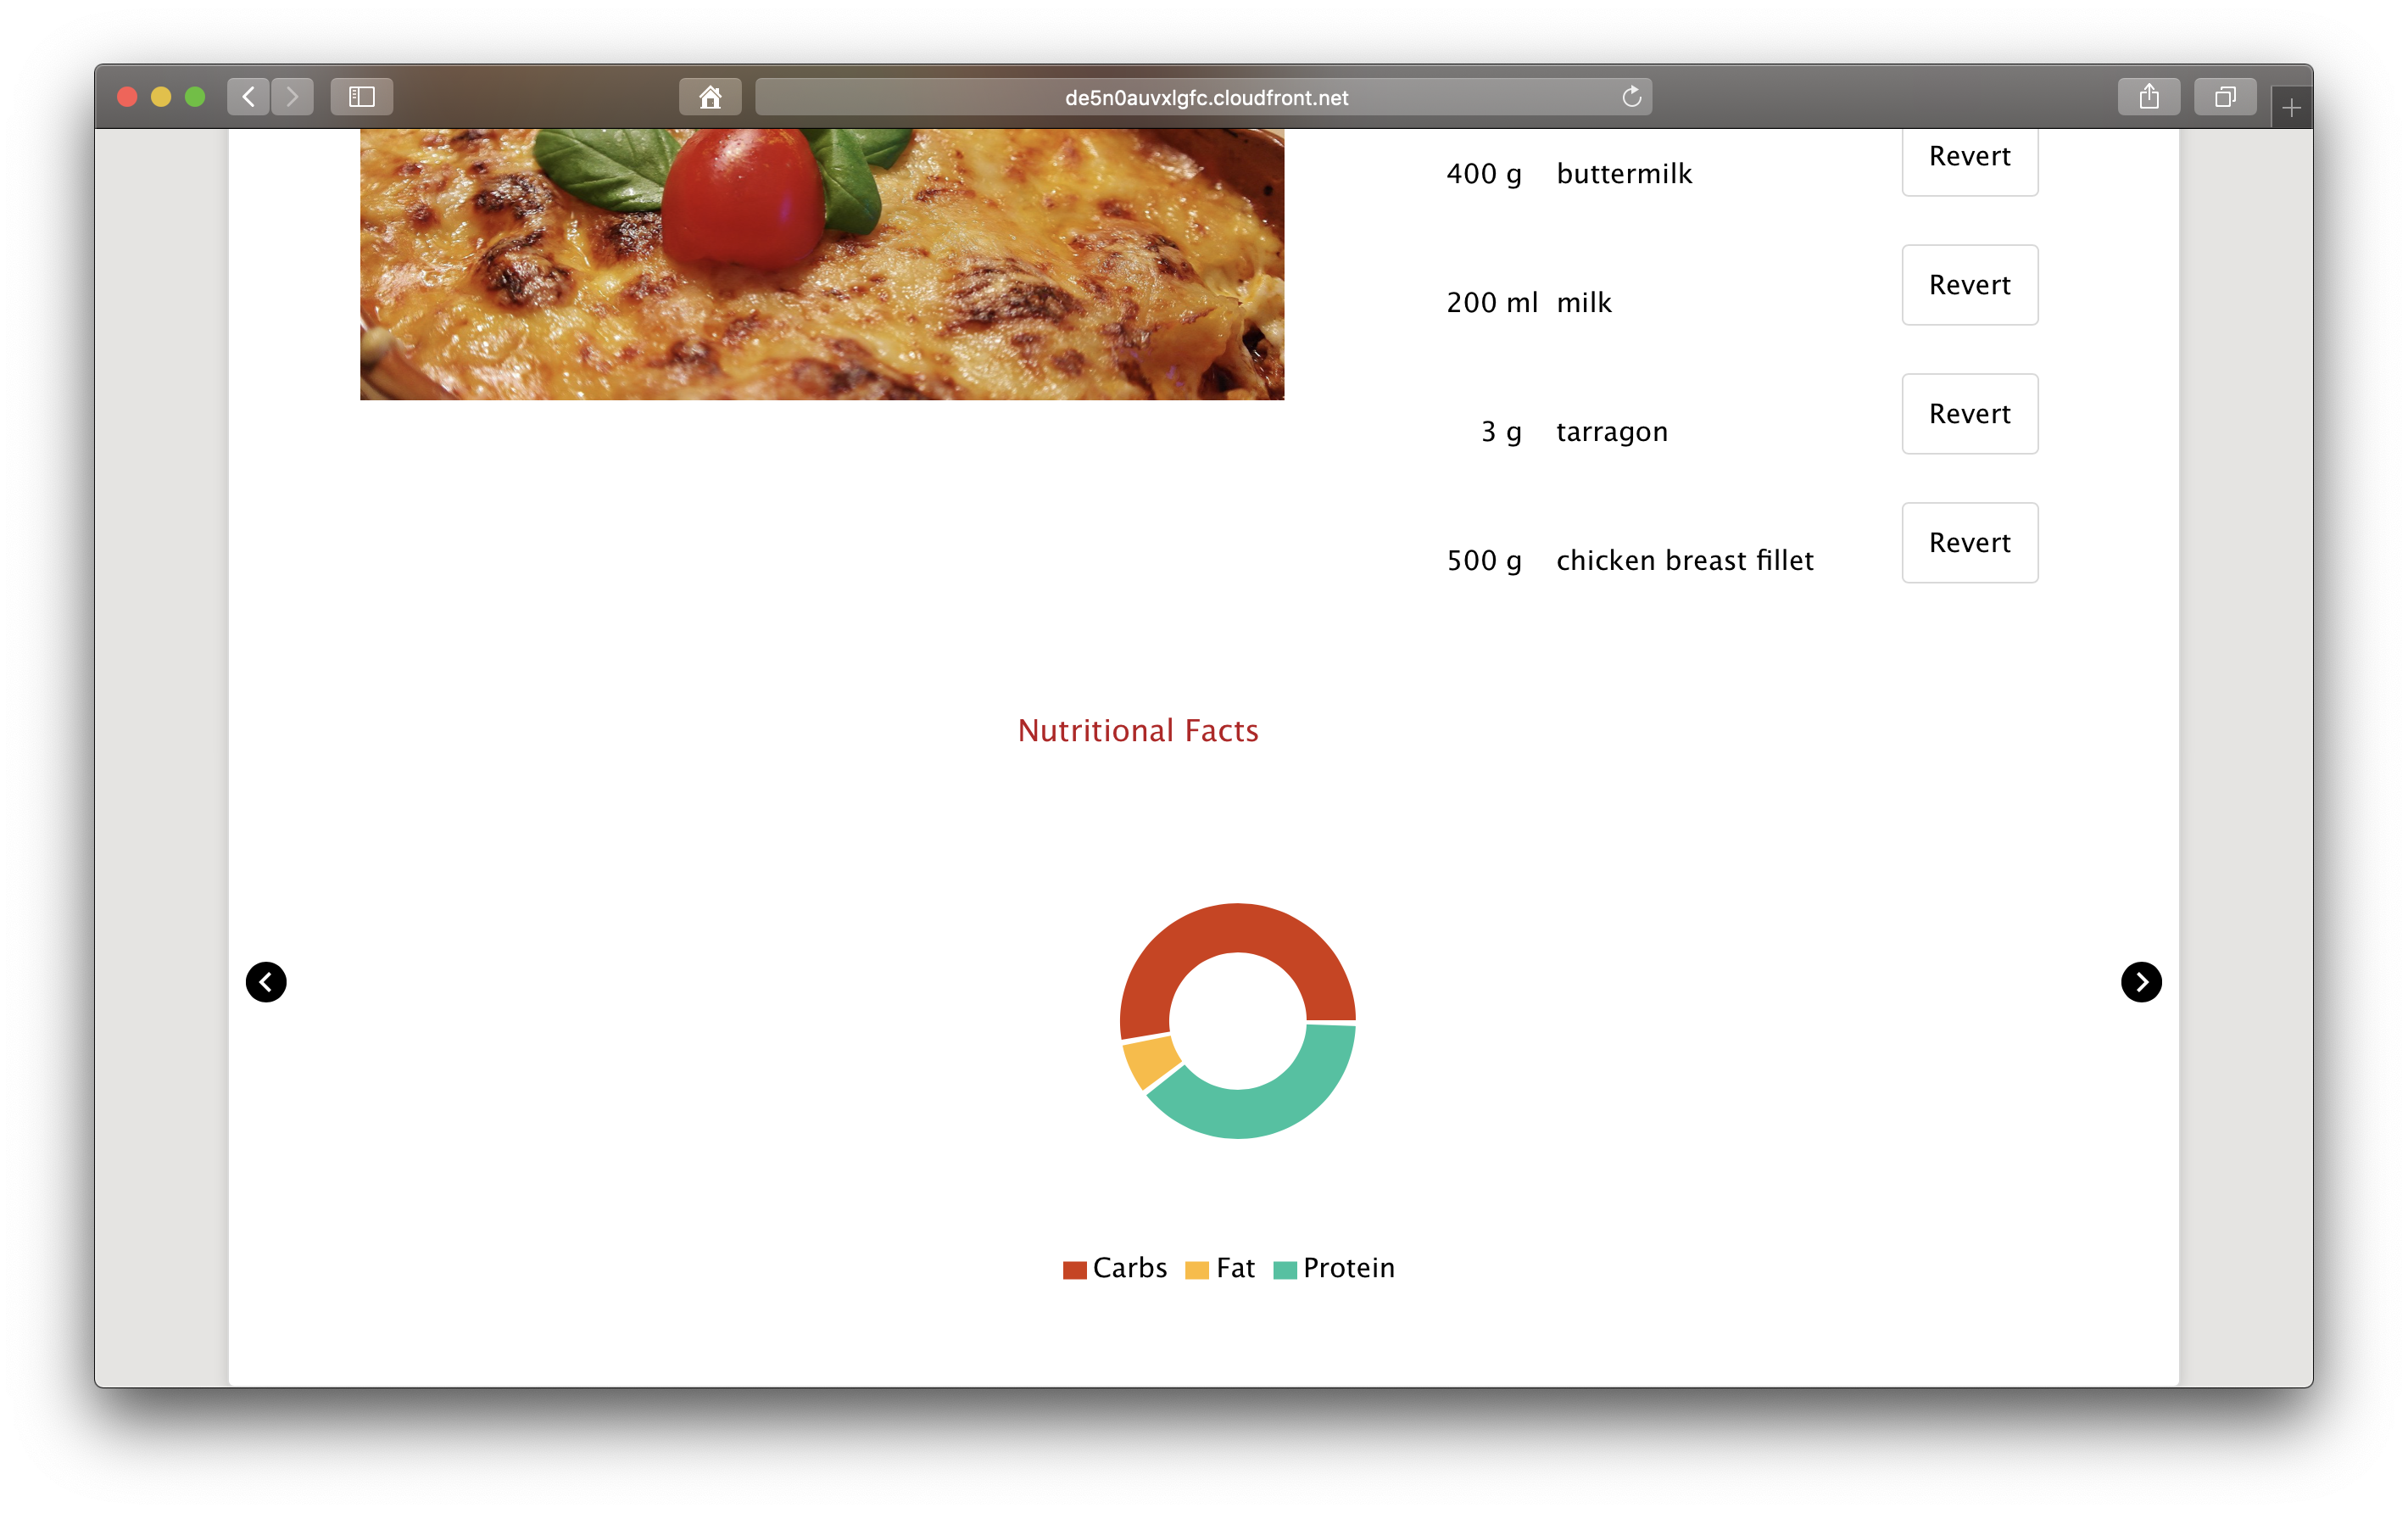
\includegraphics[scale=0.30]{Ressourcen/img/screenshots/screenshotL.png}\hfill
		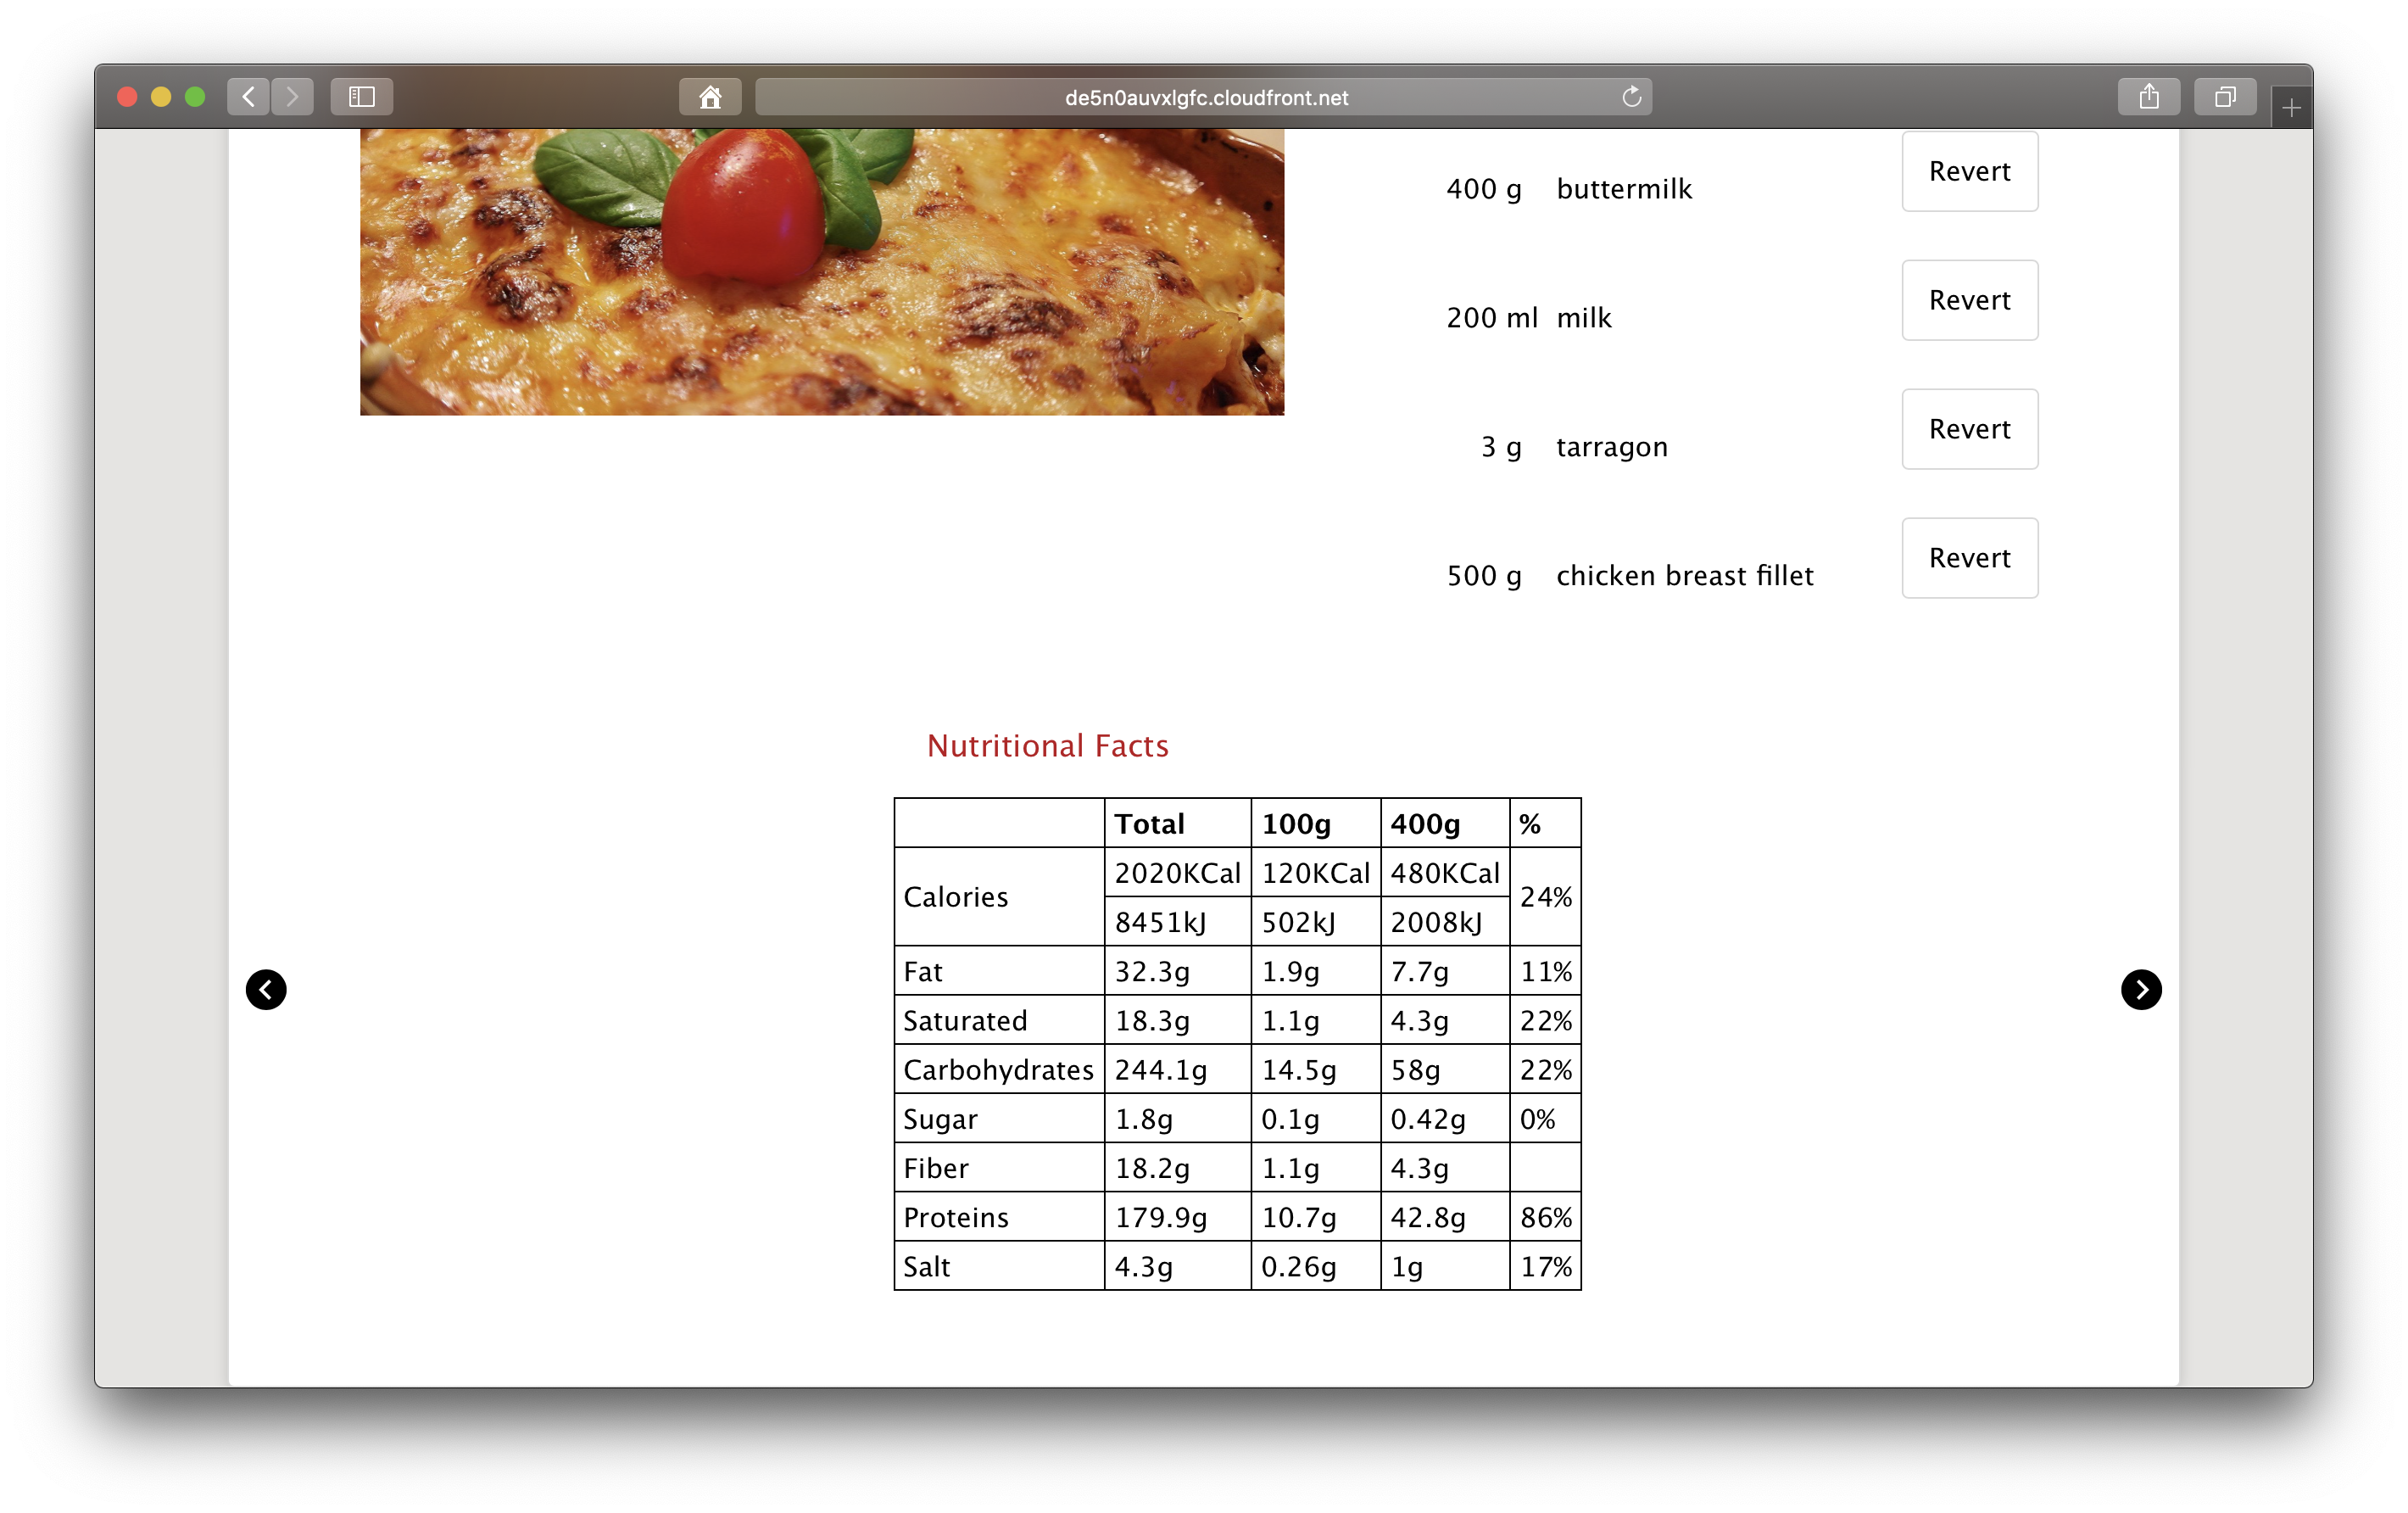
\includegraphics[scale=0.30]{Ressourcen/img/screenshots/screenshotM.png}\hfill
		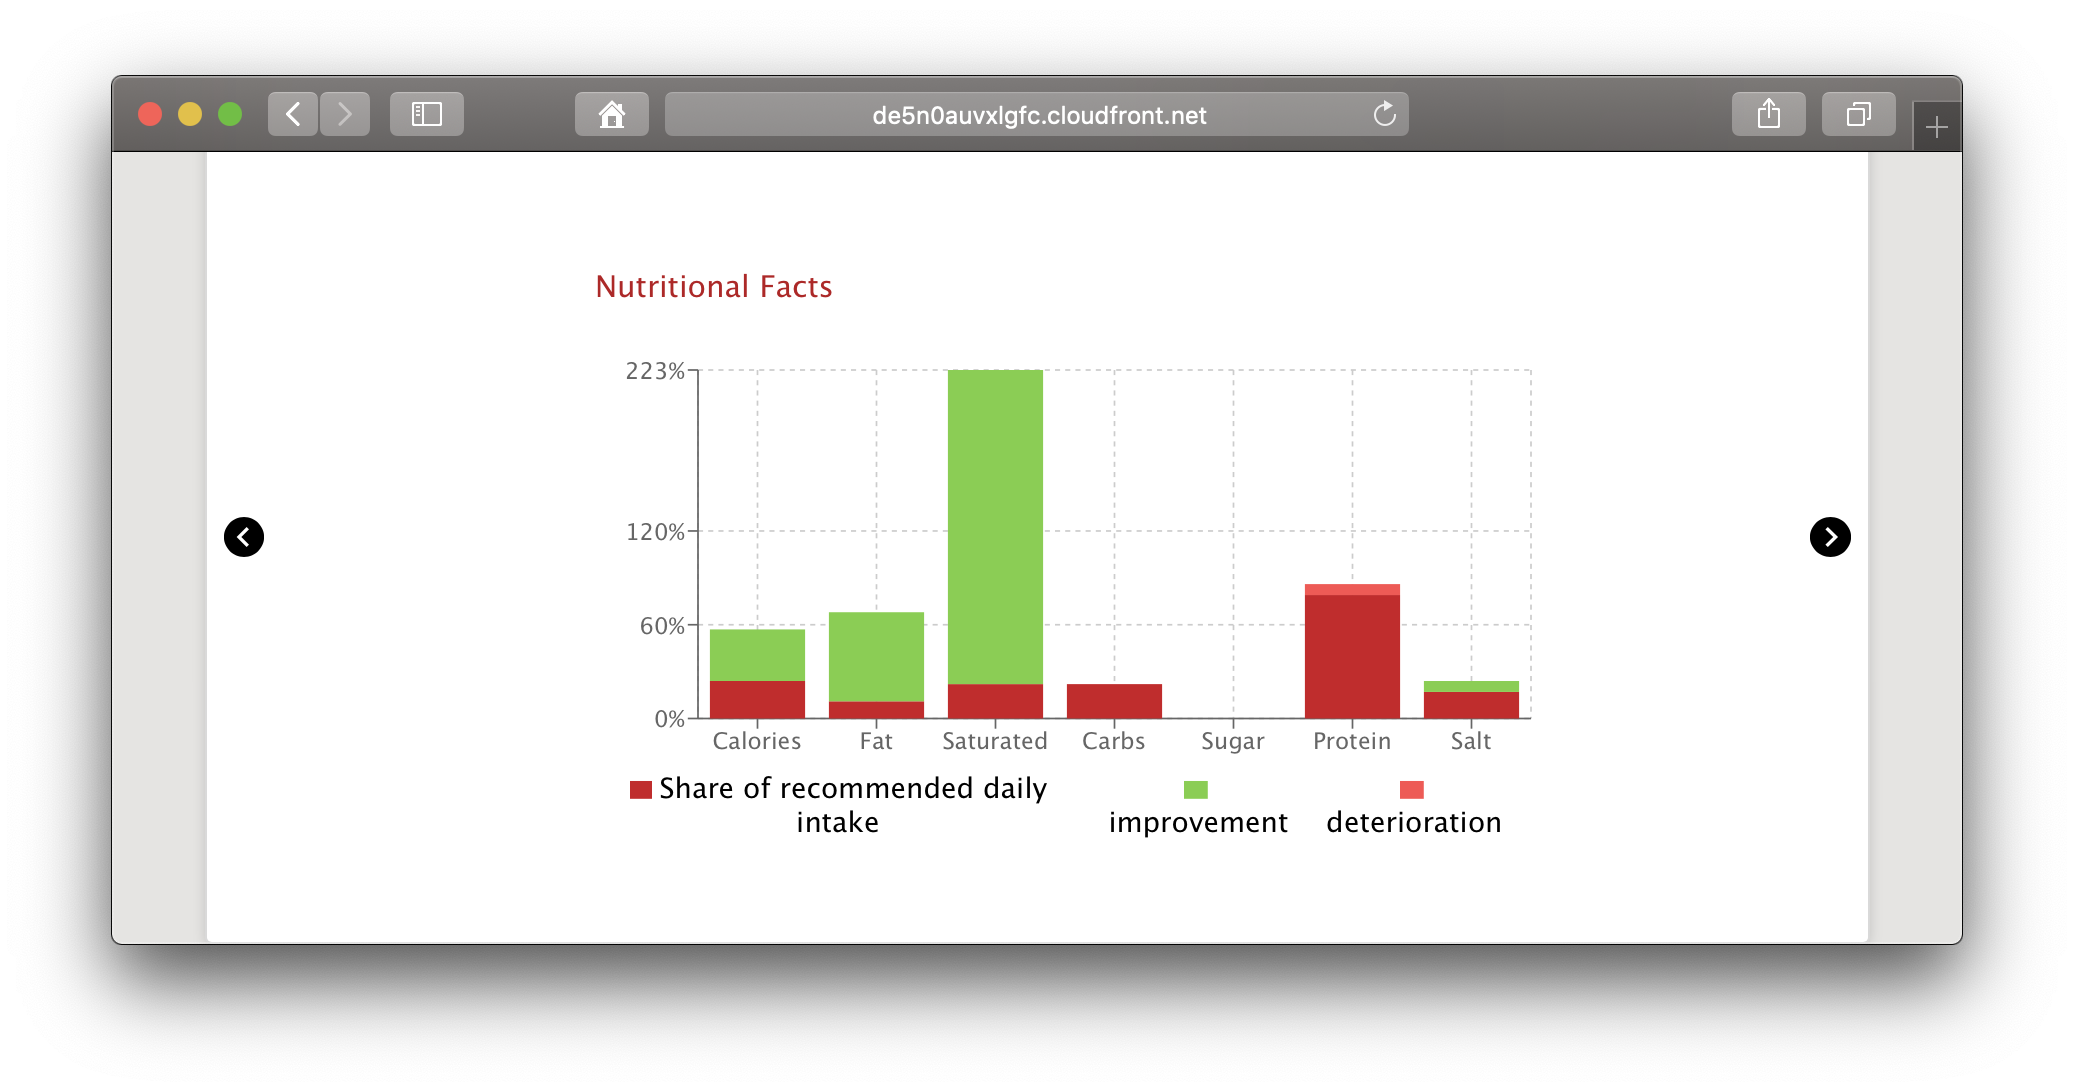
\includegraphics[scale=0.30]{Ressourcen/img/screenshots/screenshotN.png}
		\vspace{-3em}
	\end{center}
	\caption{Pie chart, table and bar graph for a recipe}
	\label{fig:detailedStatistics}
\end{figure}

\section*{Profile Page}

\vspace{-1em}
\begin{figure}[H]
	\captionsetup{justification=centering}
	\begin{center}
		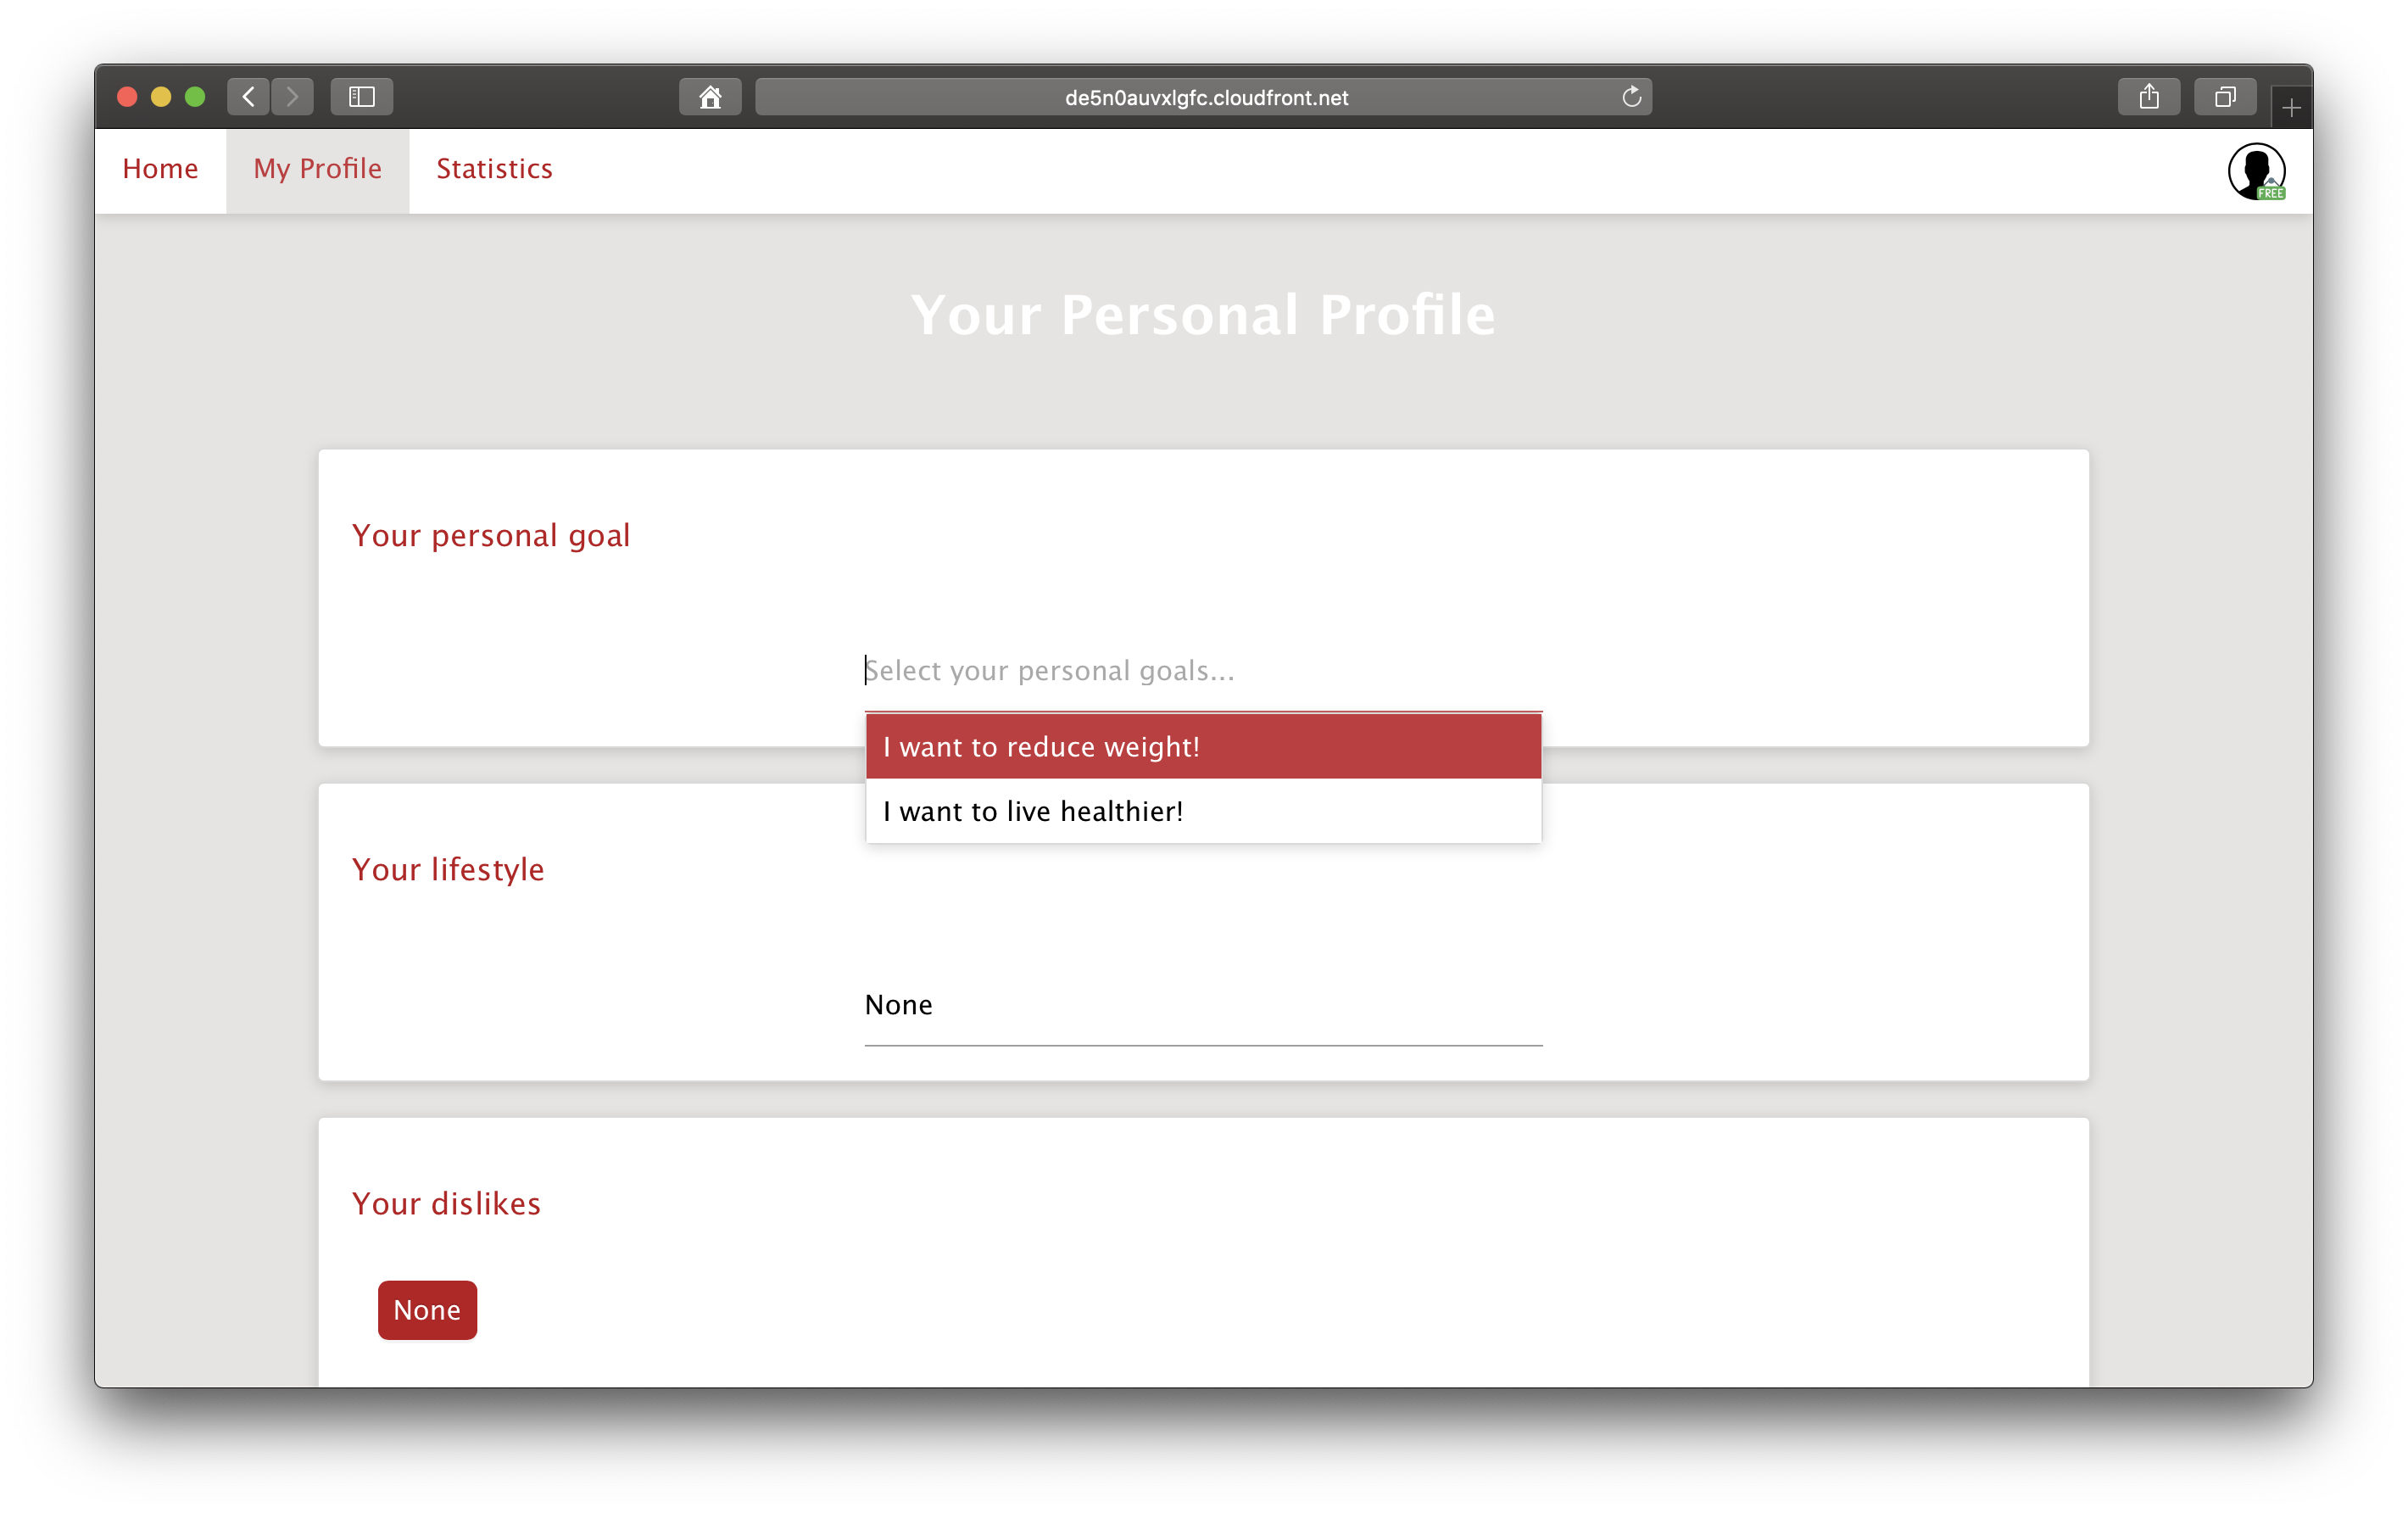
\includegraphics[scale=0.25]{Ressourcen/img/screenshots/screenshotO.png}
		\vspace{-2em}
		\caption{Profile page goal and lifestyle}
	\end{center}
\end{figure}
\vspace{-3.5em}
As already mentioned above, the user first has to select his personal goal before he can use the substitution service. To improve the received substitutes from the substitution algorithm, it is advised for the user to also insert additional personal information, currently consisting of:
\vspace{-3em}

\begin{itemize}
\item \textbf{Goal}: Reduce weight or live healthier.
\item \textbf{Lifestyle}: Vegetarian, low carb or vegan
\item \textbf{Dislikes}: A list of ingredients he does not like and therefore wishes to not be shown as substitutes.
\item \textbf{Allergies}: A list of ingredients he can not eat and therefore should not be shown as substitutes.
\end{itemize}
\vspace{-1em}
Changes to a user’s profile will be saved automatically and can always be changed again.
\vspace{-1em}

\begin{figure}[H]
	\captionsetup{justification=centering}
	\begin{center}
		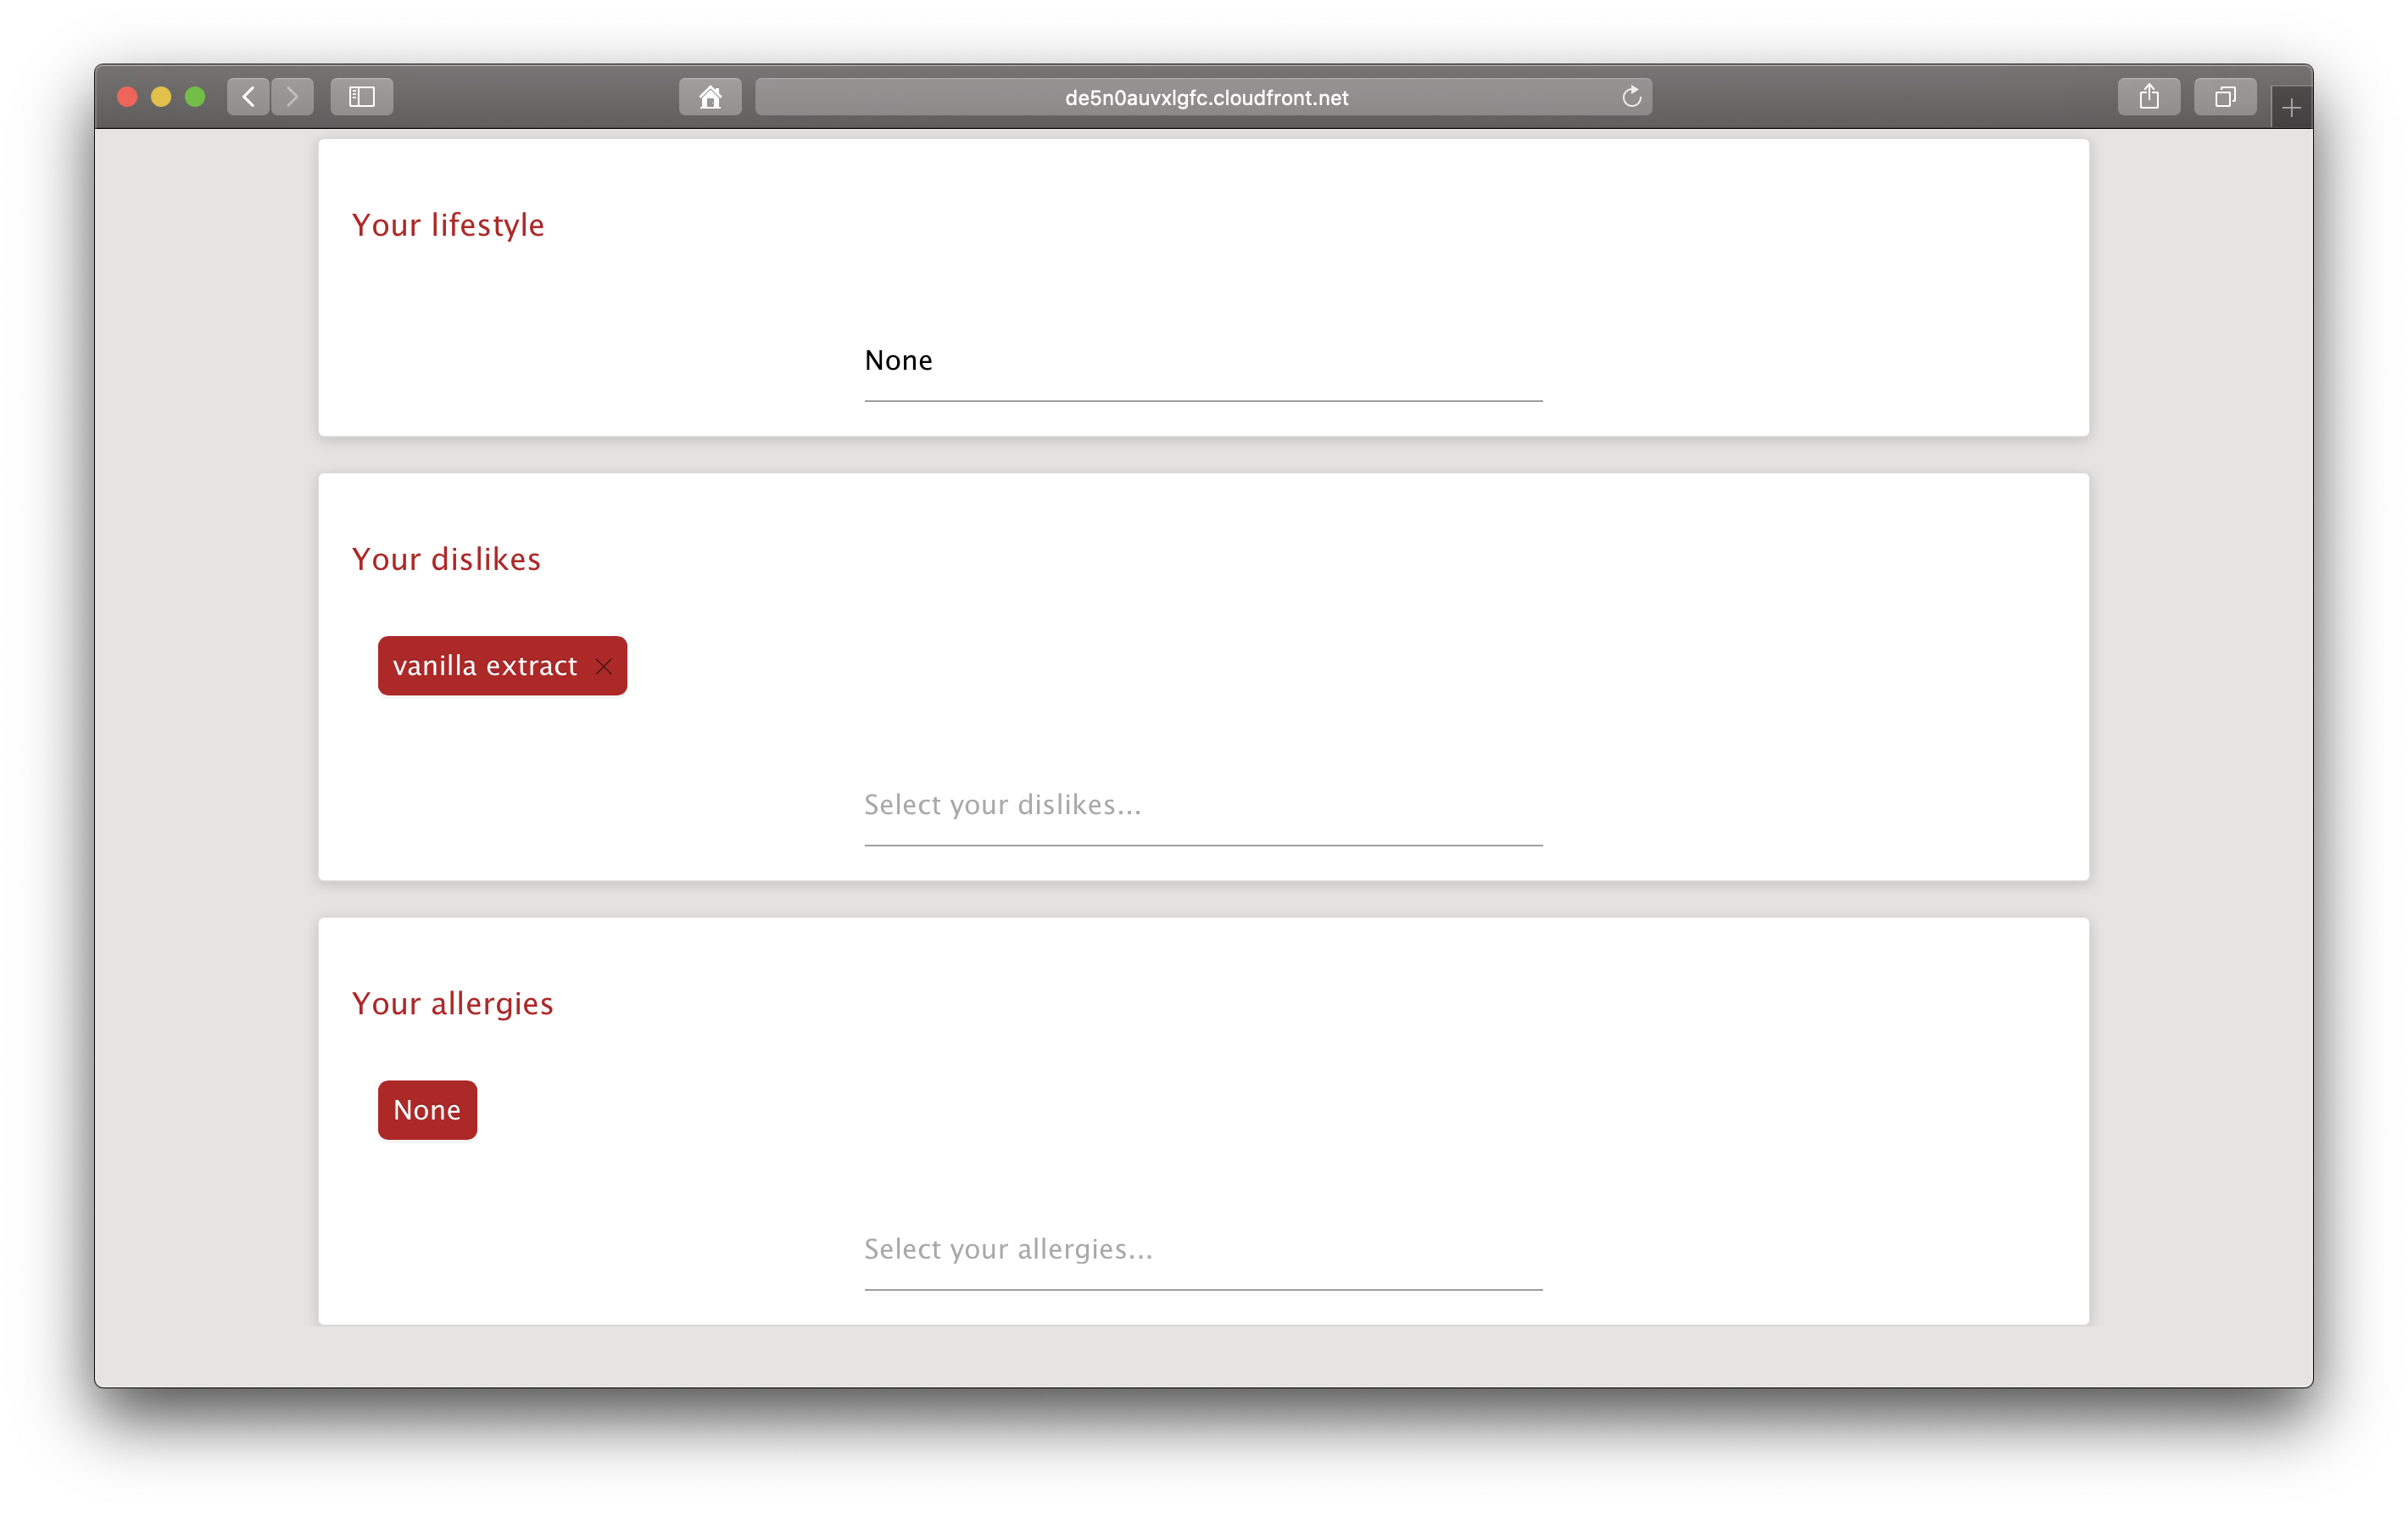
\includegraphics[scale=0.25]{Ressourcen/img/screenshots/screenshotP.png}
		\vspace{-2em}
		\caption{Profile page dislikes and allergies}
	\end{center}
\end{figure}

\section*{Statistics Page}
\vspace{-2em}
\begin{figure}[H]
	\captionsetup{justification=centering}
	\begin{center}
		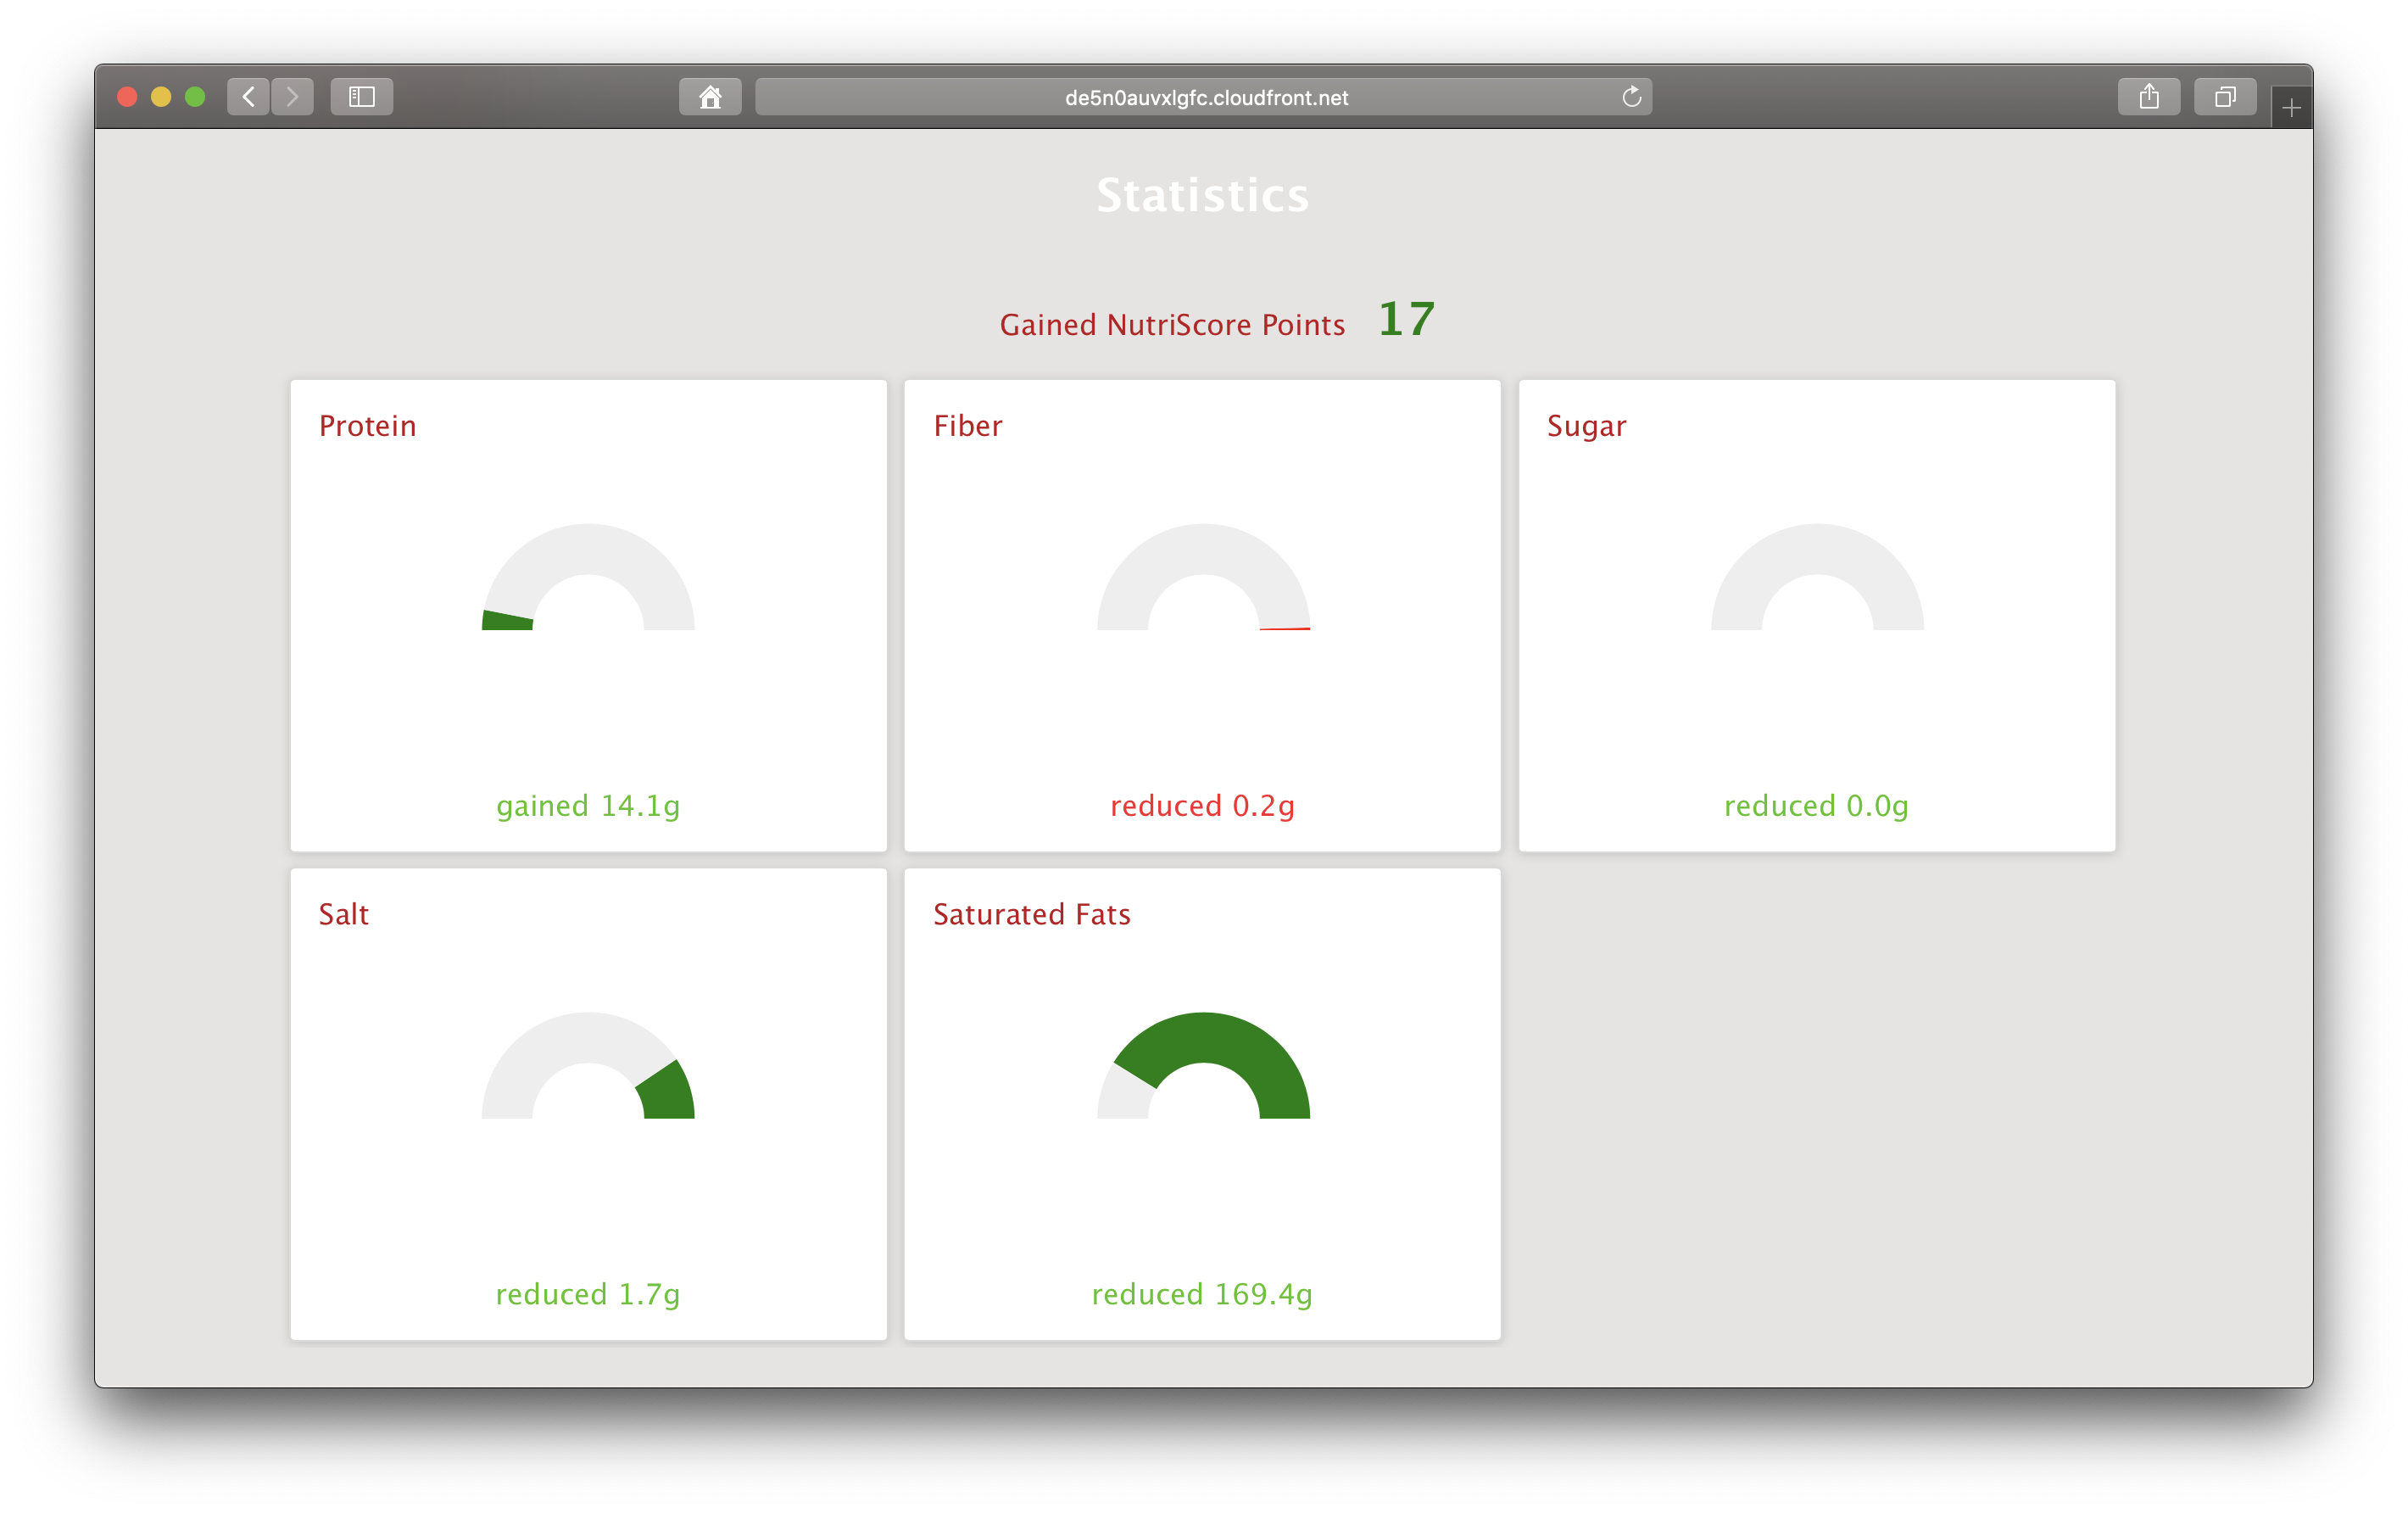
\includegraphics[scale=0.30]{Ressourcen/img/screenshots/screenshotQ.png}
		\vspace{-3em}
		\caption{User statistics}
	\end{center}
\end{figure}
By clicking on \texttt{Statistics} in the navbar, a user can get an overview about his nutritional career with Foodo. Throughout his substitution history, some personal nutritional data will be gathered and stored for each user. He can see how many NutriScore points he improved his recipes in total, as well as the amount of the five main nutritional values. Improvements, such as gaining protein or fiber and reducing sugar, salt or saturated fats, will be highlighted in green while negative changes will be highlighted in red.

\section*{PayPal Premium}
\vspace{-2em}
\begin{figure}[H]
	\captionsetup{justification=centering}
	\begin{center}
		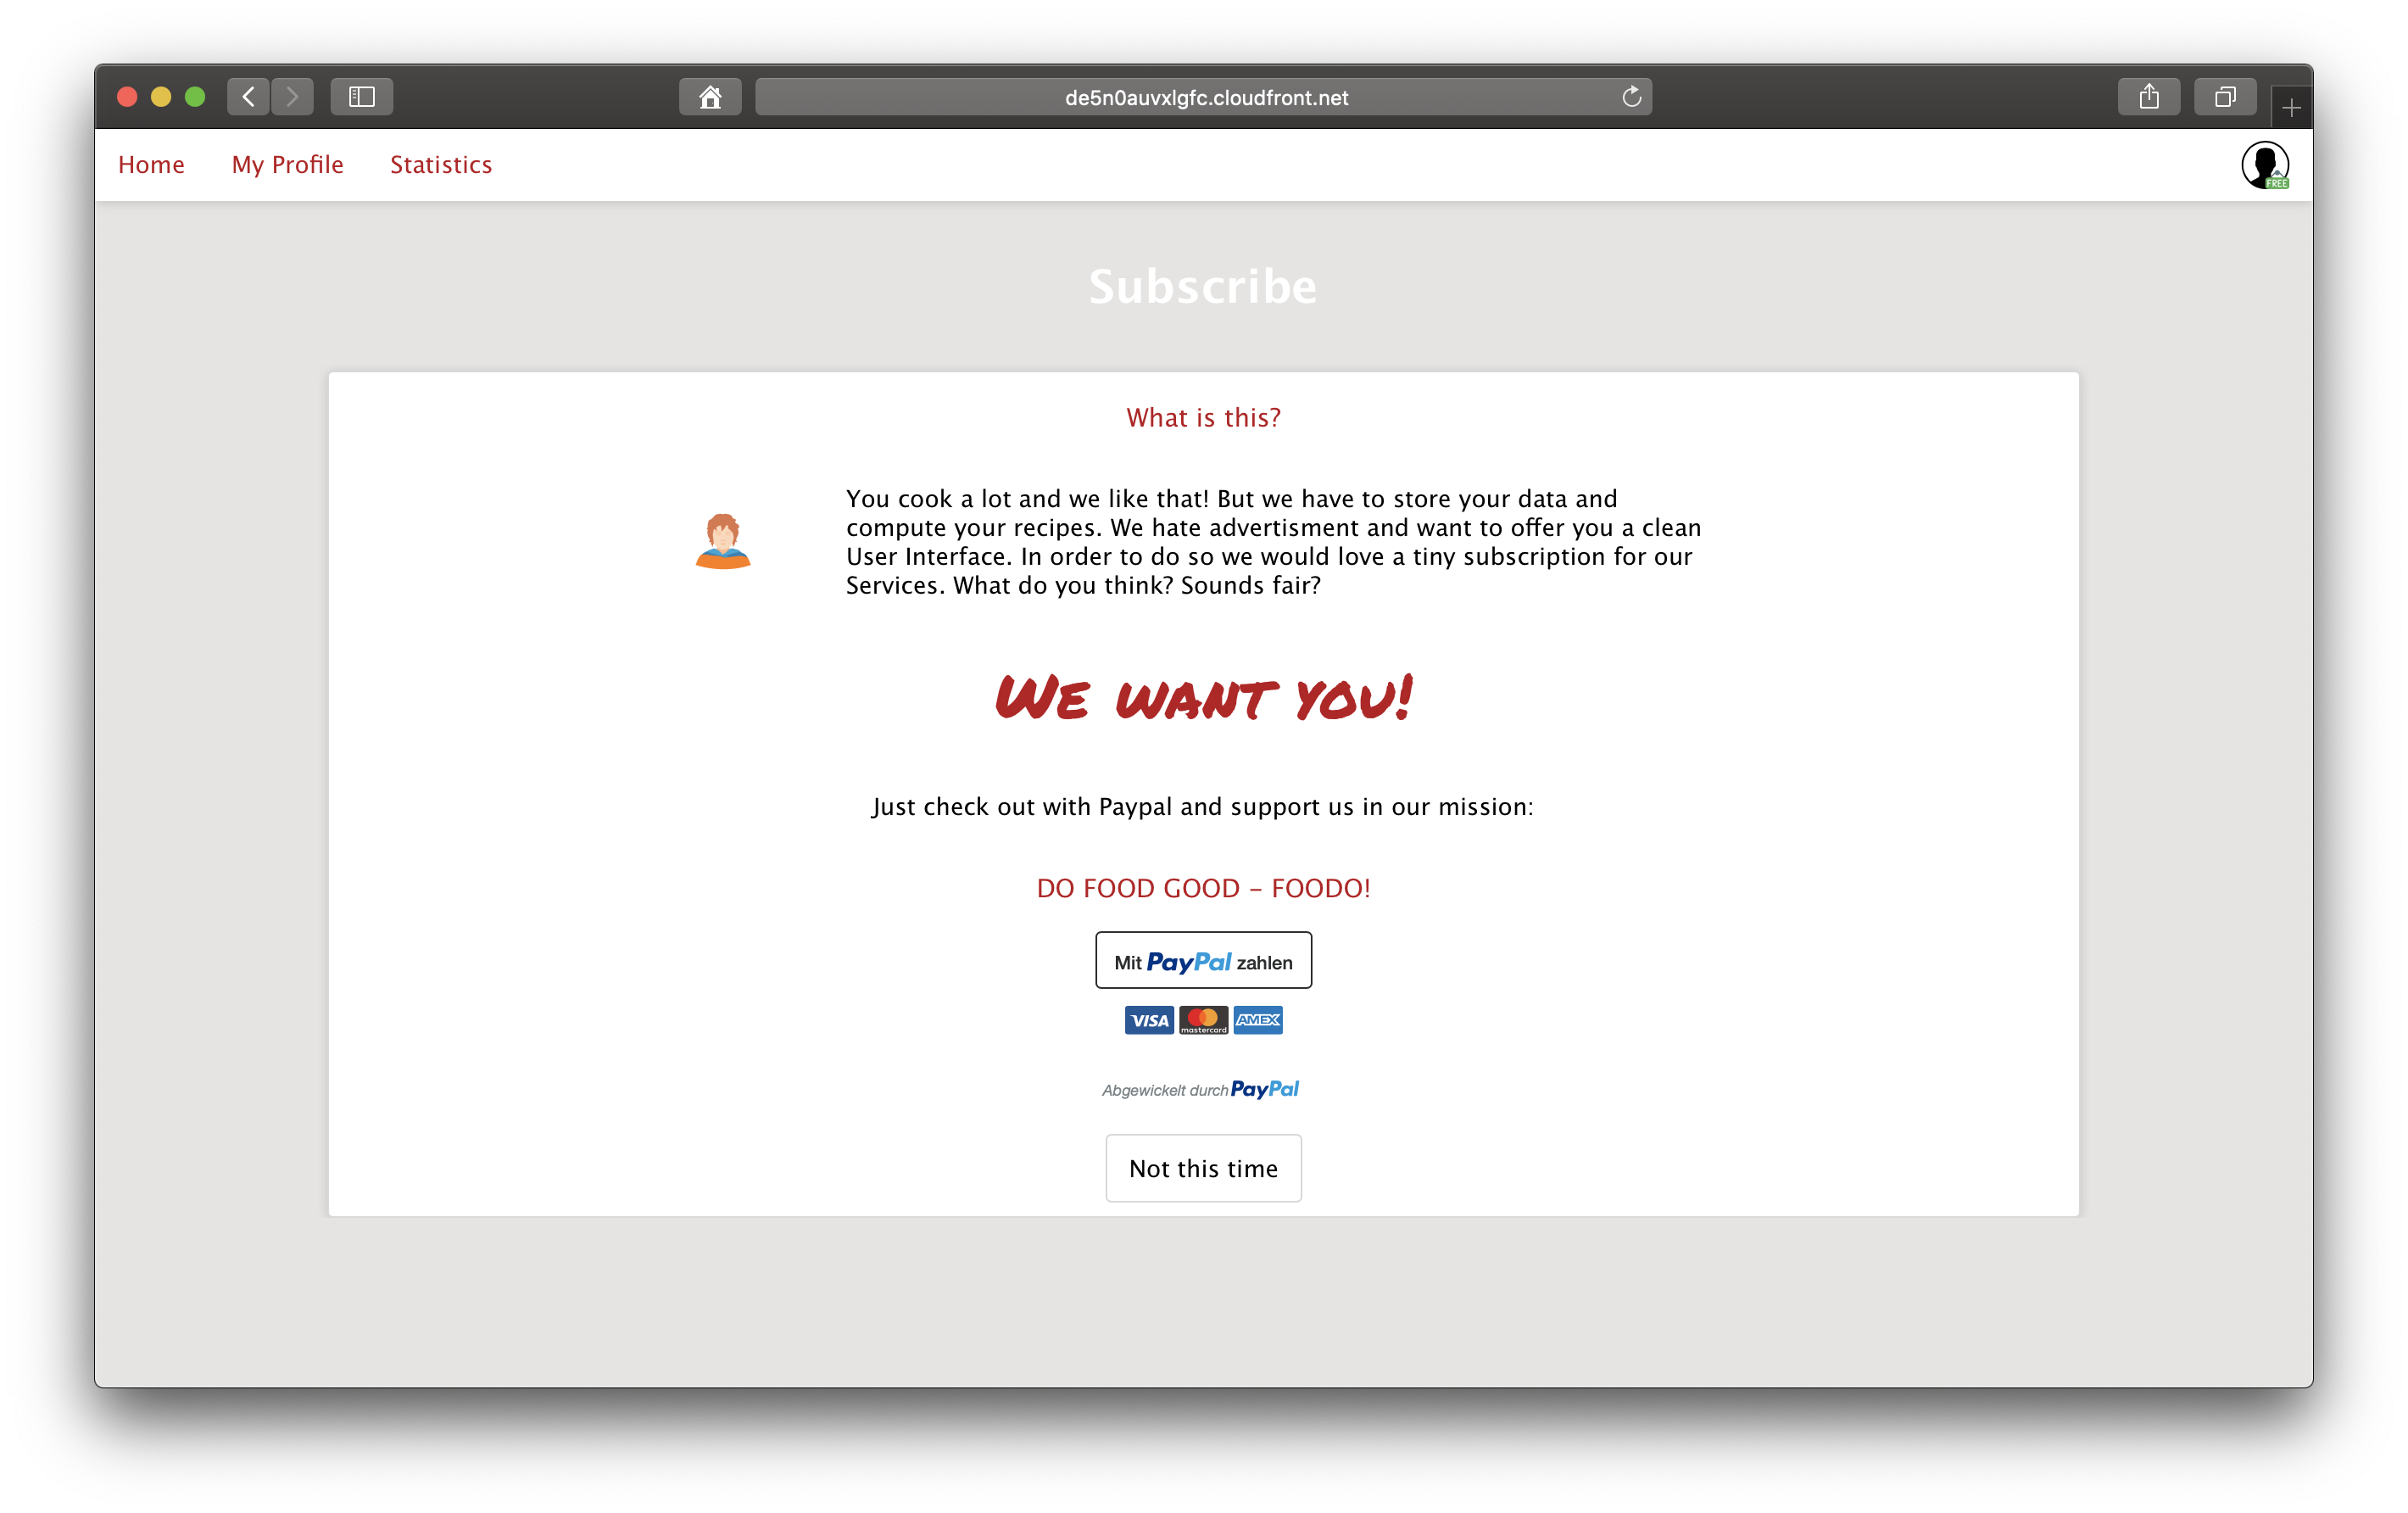
\includegraphics[scale=0.25]{Ressourcen/img/screenshots/screenshotR.png}
		\vspace{-2em}
		\caption{Premium opportunity}
		\label{fig:paypal}
	\end{center}
\end{figure}
From time to time, the user will see the popup shown in figure \ref{fig:paypal}, where he can acquire a premium status. This will change the \texttt{Free} label next to the profile icon in the upper right corner to a star and will help the developer team to implement additional features.
\clearpage
\section*{Mobile Version}
Foodo is also available for all mobile devices with access to a web browser. Some examples are shown in the figures below.

\begin{figure}[htp]
	\captionsetup{justification=centering}
	\centering
		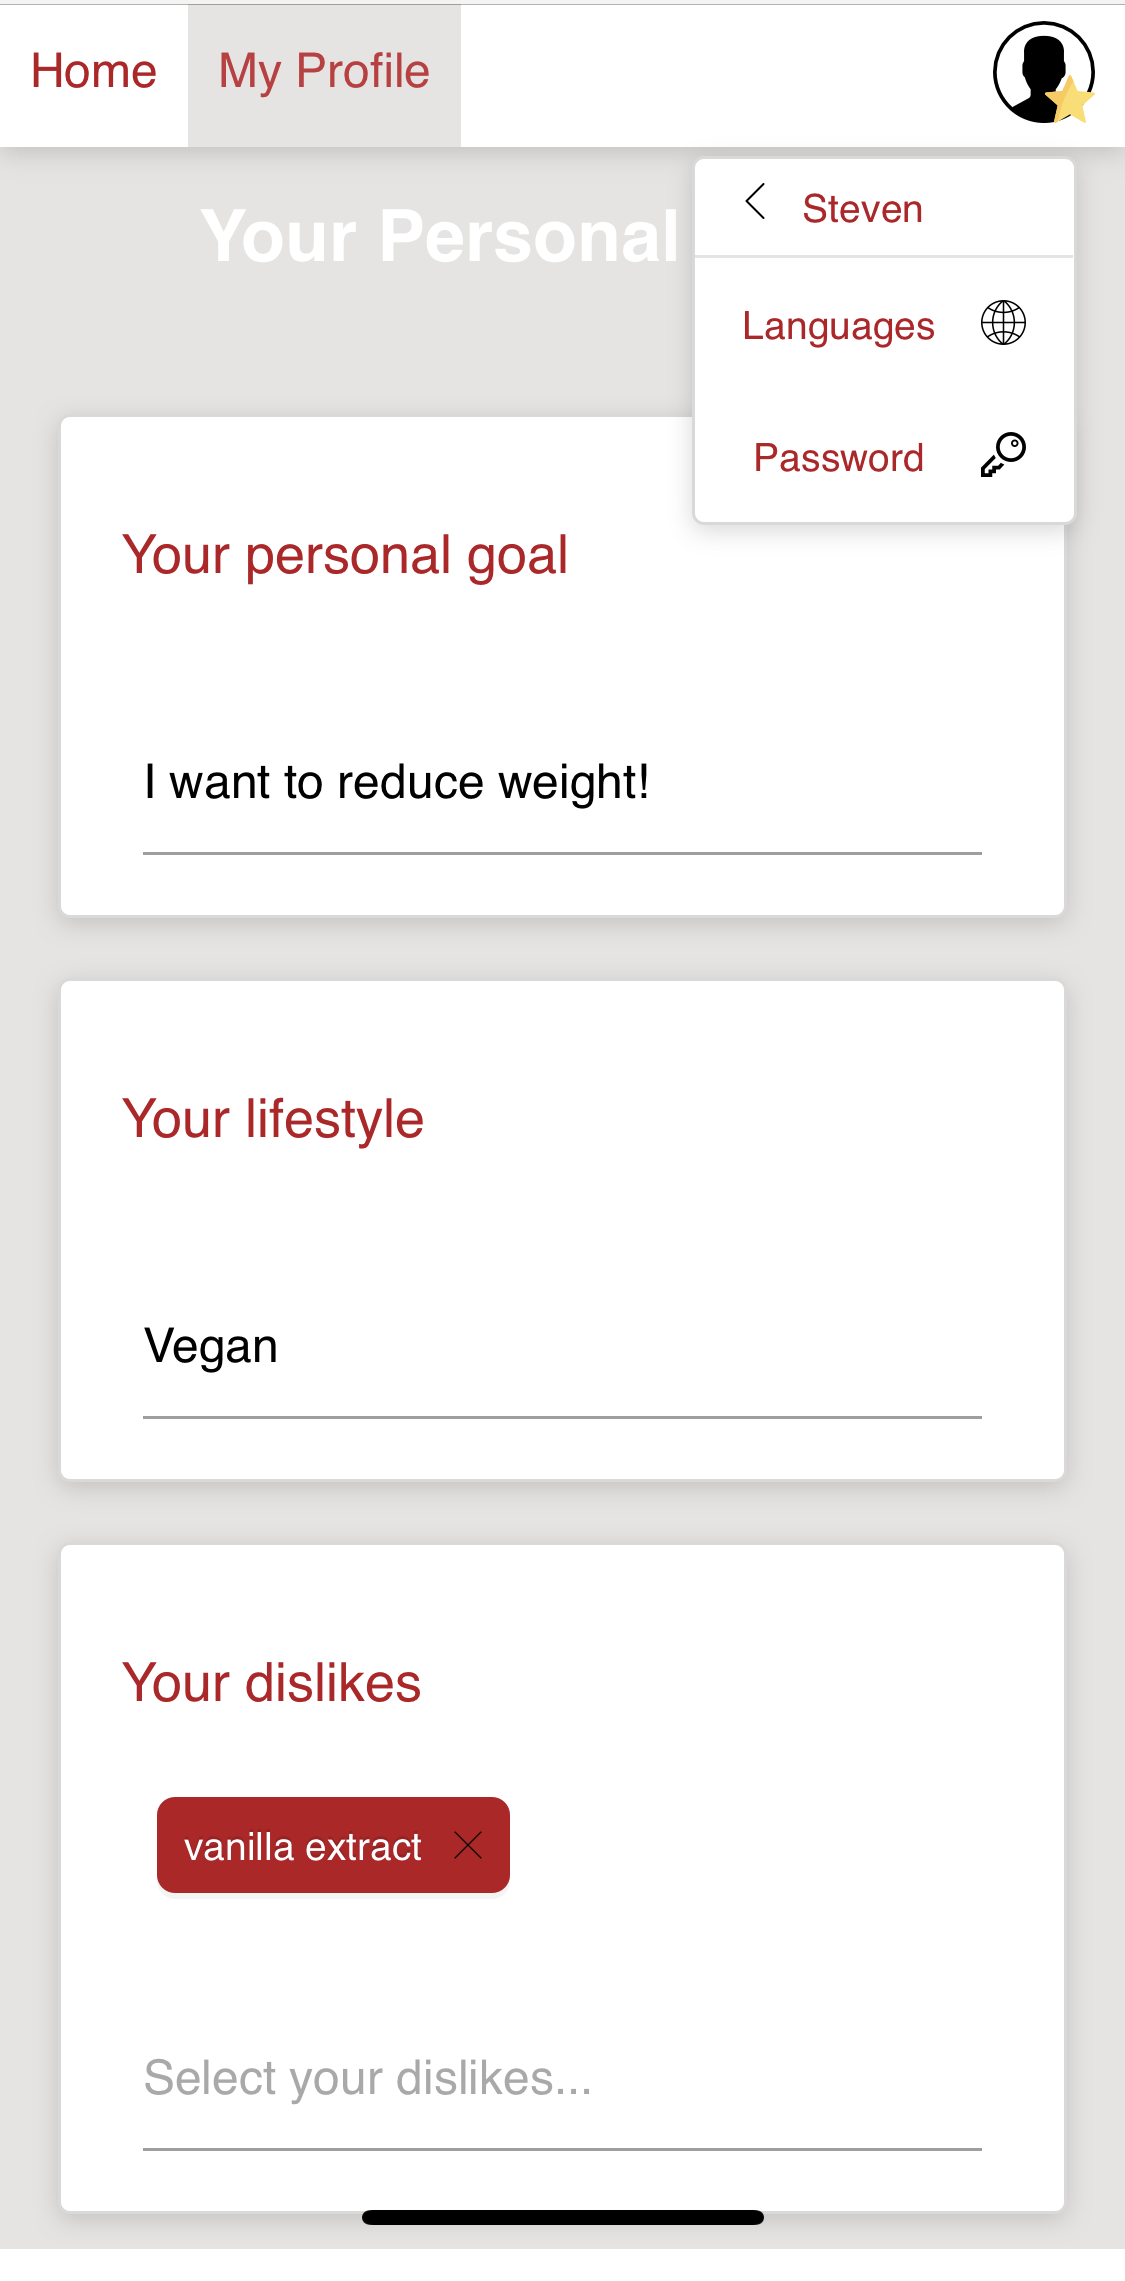
\includegraphics[scale=0.12]{Ressourcen/img/screenshots/iphone1.png}\hfill
	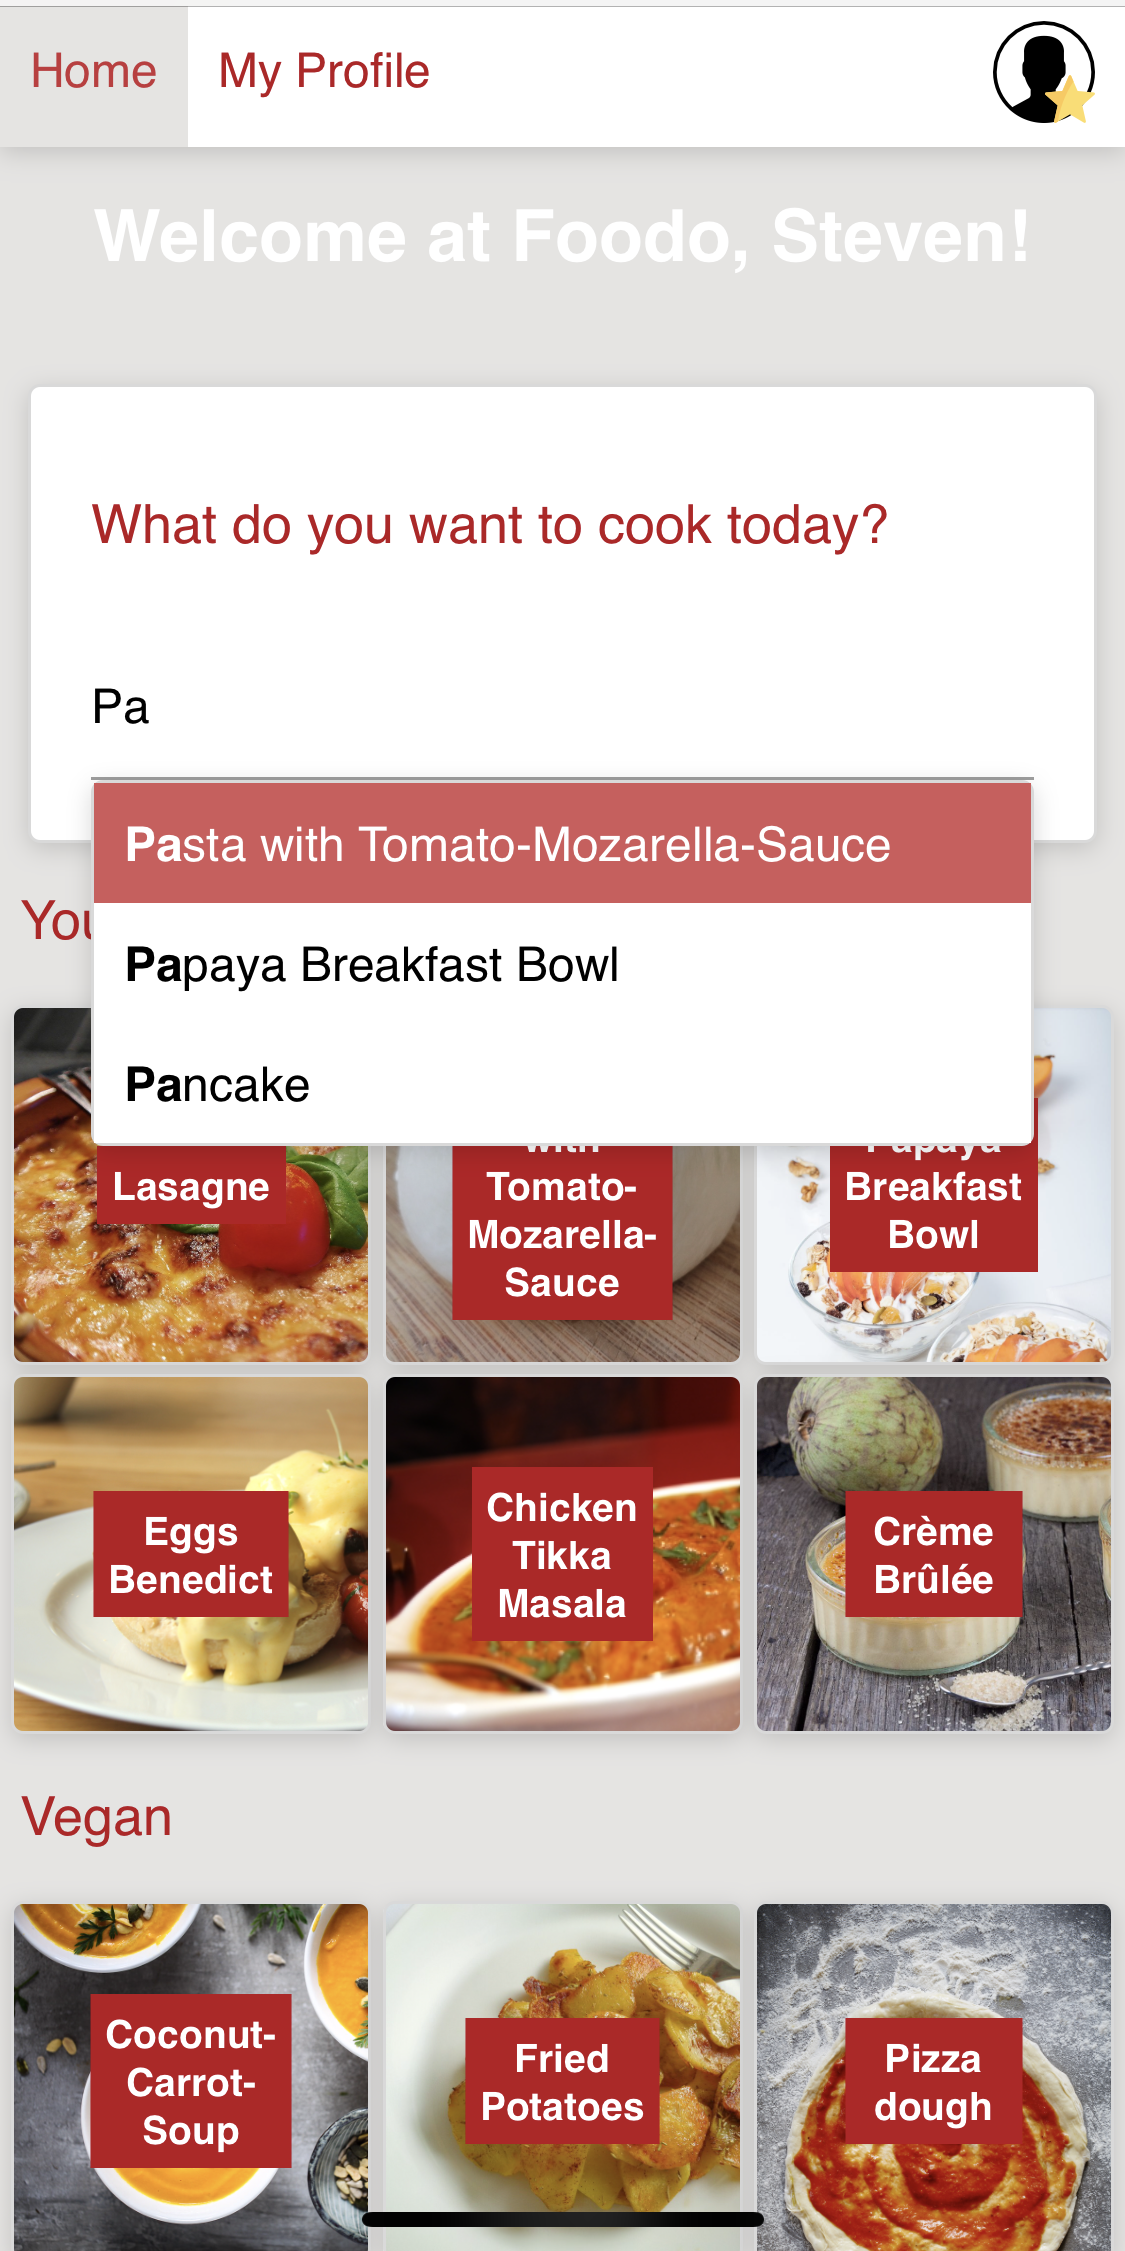
\includegraphics[scale=0.12]{Ressourcen/img/screenshots/iphone2.png}\hfill
		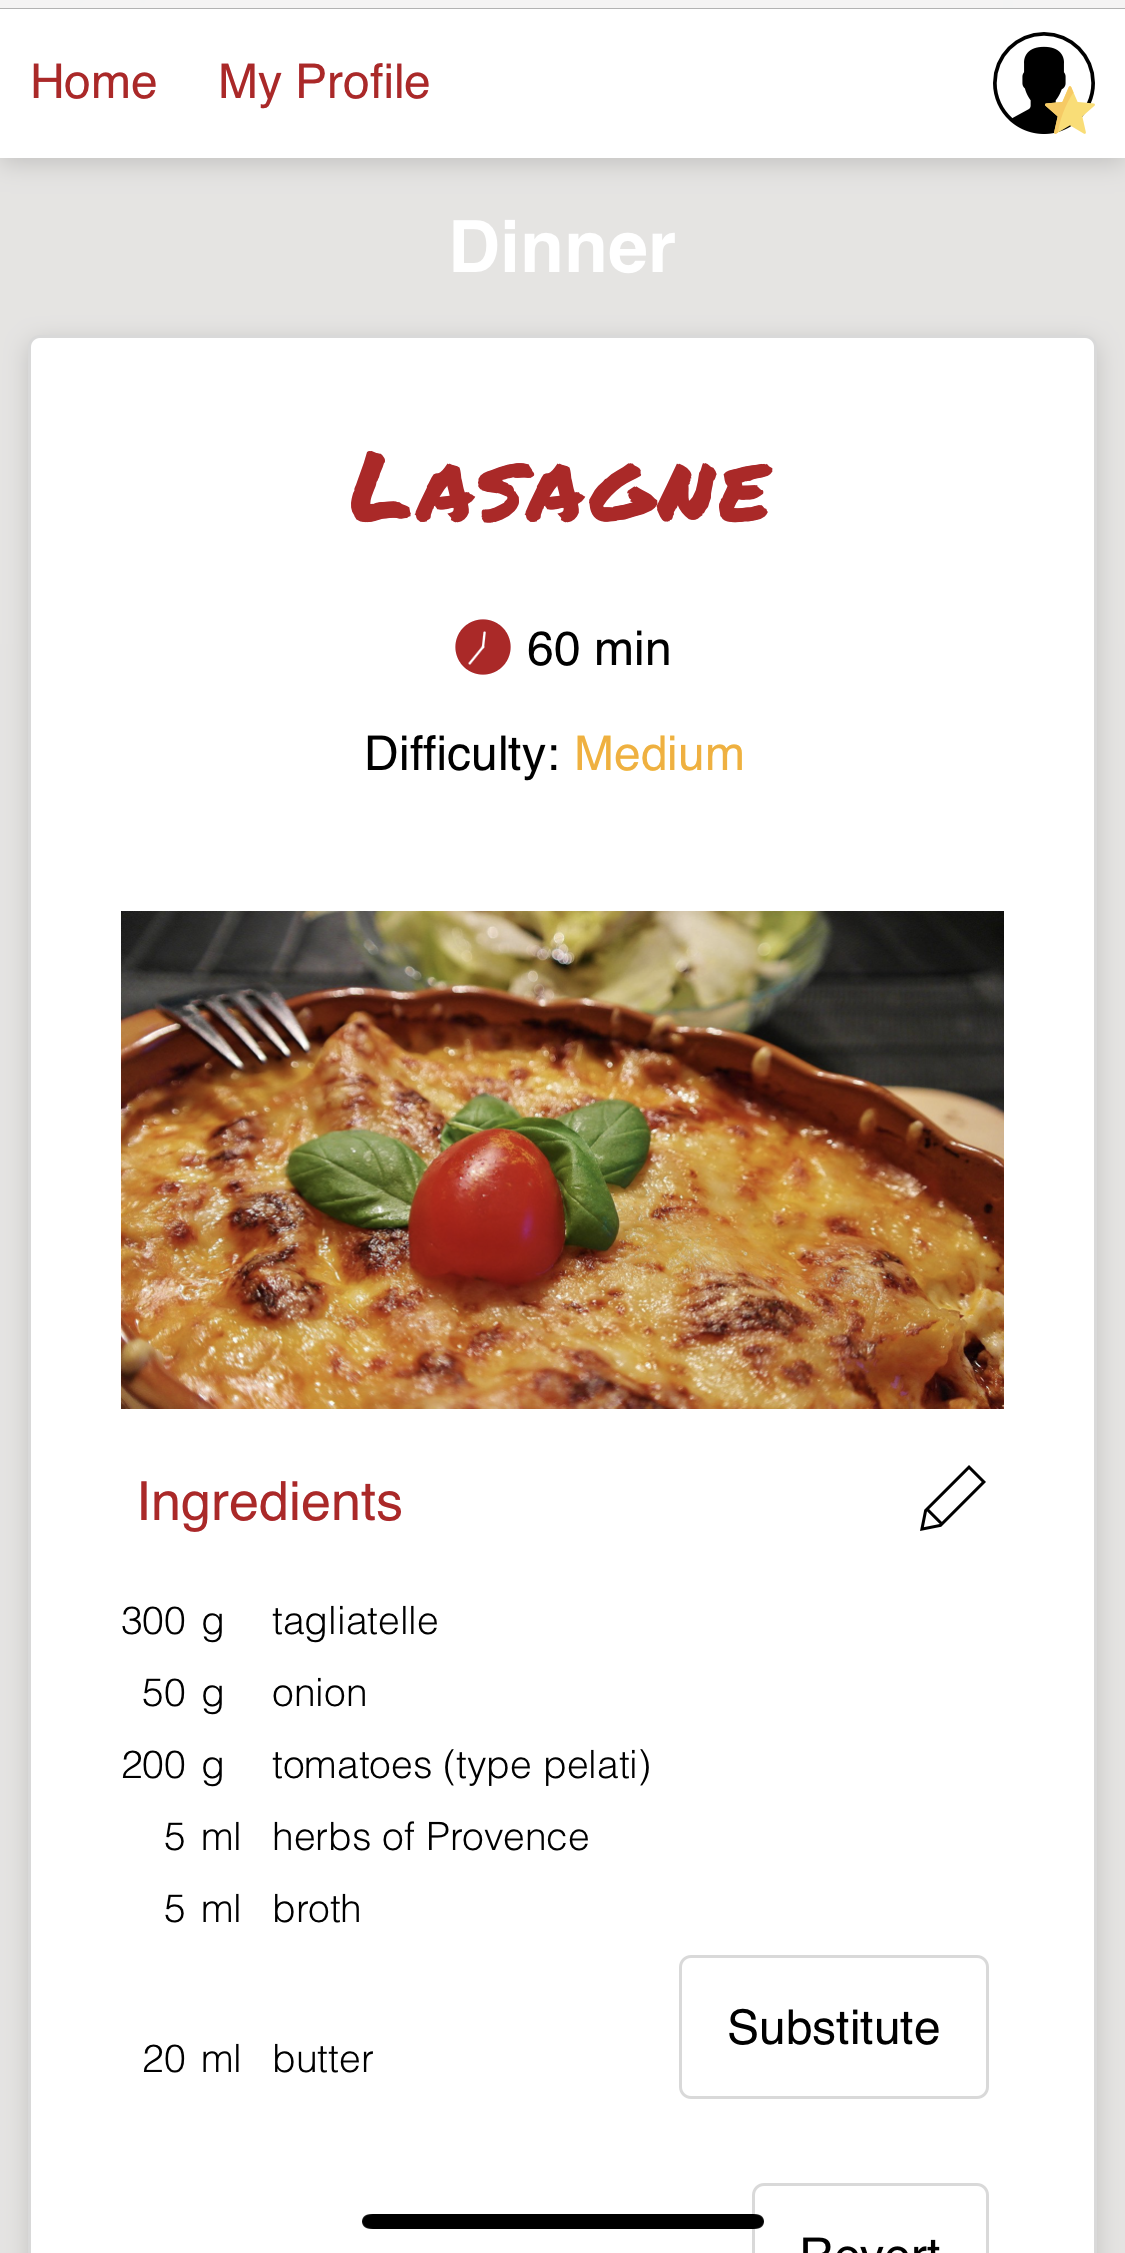
\includegraphics[scale=0.12]{Ressourcen/img/screenshots/iphone3.png}
	\caption{Mobile screenshots}
\end{figure}


